\documentclass[10pt,twocolumn,letterpaper]{article}

\usepackage{cvpr}
\usepackage{times}
\usepackage{epsfig}
\usepackage{graphicx}
\usepackage{amsmath}
\usepackage{amssymb}
\usepackage{booktabs}
\usepackage{multirow}
\usepackage{array}
\usepackage{subcaption}
\usepackage{optidef}
\usepackage{xcolor}
% Include other packages here, before hyperref.
\usepackage{alphalph}
\renewcommand*{\thesubfigure}{%
\alphalph{\value{subfigure}}%
}%

% If you comment hyperref and then uncomment it, you should delete
% egpaper.aux before re-running latex.  (Or just hit 'q' on the first latex
% run, let it finish, and you should be clear).
\usepackage[breaklinks=true,bookmarks=false]{hyperref}

\cvprfinalcopy % *** Uncomment this line for the final submission

\def\cvprPaperID{****} % *** Enter the CVPR Paper ID here
\def\httilde{\mbox{\tt\raisebox{-.5ex}{\symbol{126}}}}

%commands and things
\renewcommand{\vec}[1]{\mathbf{#1}}
\newcommand{\Real}[1]{\mathbb{R}^{#1}}
\newcommand{\ReLU}{\texttt{ReLU}\,}
\newcommand{\ReLUBN}{\texttt{ReLU + BN}\,}
\newcommand{\moons}{\texttt{MOONS}\,}
\newcommand{\cifar}{\texttt{CIFAR-10}\,}
\newcommand{\SepConstraint}{\texttt{Sep-Cons}\,}
\newcommand{\SepUnit}{\texttt{Sep-U}\,}
\newcommand{\SepLayer}{\texttt{Sep-L}\,}
\newcommand{\SepPoint}{\texttt{Sep-P}\,}
\newcommand{\SepLayerBN}{\texttt{Sep-L-BN}\,}
\newcommand{\SepUnitPoint}{\texttt{Sep-P+U}\,}
\newcommand{\layer}{\ell}
\newcommand\fuck[1]{\textcolor{red}{#1}}
\DeclareMathOperator*{\argmin}{arg\,min}
\DeclareMathOperator*{\argmax}{arg\,max}

%%% theorem styles and stuff
\newtheorem{theorem}{Theorem}[section]
\newtheorem{corollary}{Corollary}[theorem]
\newtheorem{lemma}[theorem]{Lemma}
\newtheorem{remark}[theorem]{Remark}
\newtheorem{proposition}[theorem]{Proposition}
\newtheorem{definition}{Definition}[section]




% Pages are numbered in submission mode, and unnumbered in camera-ready
%\ifcvprfinal\pagestyle{empty}\fi
%\setcounter{page}{4321}
\begin{document}

%%%%%%%%% TITLE
\title{Increasing separation in units for greater perforamnce an zero initialization}

\author{Riera-Molina C.\\
Universitat de Barcelona\\
Gran Via de les Corts Catalanes 585, Barcelona Spain, 08005\\
{\tt\small blauigris@gmail.com}
% For a paper whose authors are all at the same institution,
% omit the following lines up until the closing ``}''.
% Additional authors and addresses can be added with ``\and'',
% just like the second author.
% To save space, use either the email address or home page, not both
\and
Rey-Torres C.\\
Universitat de Barcelona\\
Gran Via de les Corts Catalanes 585, Barcelona Spain, 08005\\
{\tt\small camilorey@gmail.com}
}

\maketitle
%\thispagestyle{empty}

\section{Introduction}\label{sec:introduction}
The success of Deep Learning has been linked to its ability to learn \emph{abstract representations} from input data in a hierarchical fashion, that reshape and resignify data as it traverses deeper into the network. Under this assumption, the deeper a DNN, the richer these representations become and the more sophisticated are the patterns learned by it \cite{LeCun06atutorial,ramachandranEtAl2017SearchingForActivationFunctions}. However, depth is also instrumental in the development of various DNN \emph{issues} like the \emph{vanishing gradient} as presented in \cite{vanishing1} or \cite{vanishing2}; the \emph{exploding gradient} as presented in \cite{exploding}; the \emph{dead unit problem} as presented in \cite{leaky},\cite{whyreludie} or \cite{whenneuronsfail}; or the \emph{degradation problem} as presented in \cite{resnet}. 
\\\\
Existing methods attempt to fix these issues by reshaping abstract representations using a variety of approaches   comprising two families, summarized for the reader in Table \ref{tab:techniquesTable}: (1) \emph{architectural modifications} and (2) \emph{data manipulations}. By architectural modifications we mean methods that profit from the feed-forward structure of DNN (i.e. function composition) to secure meaningful abstract representations by increasing for example layer width, using information from previous layers to creating additional connections within a DNN \cite{resnet,densenet}; or modifying unit activation functions to avoid trivial values \cite{crelu}. Meanwhile \emph{data manipulation} (final row of \ref{tab:techniquesTable}) attempts to somehow \emph{correct} abstract representations via covariance shifting (i.e. standarization) \cite{batchnorm} to secure coherency and numerical stability while in training. 
\\\\
In the case of \ReLU based DNN, these issues can be related to abstract representations within a \emph{geometric mindset}. More specifically, both gradient issues and unit problems are deeply intertwined with the position of the hyper-planes defined by the preactivation in \ReLU units. That is, as units partition input data, a portion of it is mapped to zero (in the negative hemi-space of the hyper-plane) while the other is forwarded affinely for further processing. Since loss gradient is only non-zero on forwarded points \cite{reyRiera2019ModellingClassificationReLU}, the vanishing gradient and dead unit problem can be traced back to \emph{improper} plane positioning, while the exploding gradient and degradation can be related to the compositions of affine forwarding in feed-forwarding DNN. We suggest that the if not managed, the issue becomes critical in \emph{deeper} DNN.   
\\\\
We contend that \emph{influencing} abstract representation evolution (while training) may secure \emph{proper separations} of data comprising an alternate method to attack aforementioned issues that neither tampers with the feed-forward structure of DNN, nor requires \emph{post-hoc} geometric transformations on data (see the final row on table \ref{tab:techniquesTable}). Moreover, we argue that an elegant approach to abstract representation regulation can be done by introducing minimizing constraints over pre-activations (during training) to secure proper plane positioning: the \texttt{Sep} constraints, over DNN parameters (as detailed throughout section \ref{sec:constraint}).
\\\\
Furthermore, our \texttt{Sep} constraints can be enforced at unit (\texttt{Sep-U}), data point (\texttt{Sep-P}) and layer level (\texttt{Sep-L}). The rationale to formulate them is derived from the explanation model constructed by Rey-Torres et al. in  \cite{reyRiera2019ModellingClassificationReLU} as detailed in section \ref{sec:separability}. 
\\\\
Throughout section \ref{sec:experiments} we test our separation constraints on the \texttt{MOONS} dataset in a series of experiments, that increase our insight into the mechanics and dynamics of separation performed by a deep DNN and the effect of  separation constraints, and benchmark it to batch-normalization.  

\begin{table*}[h!]
\centering
\begin{tabular}{@{}llll@{}}
\toprule
Family & Method & Examples & Intended issues\\ 
\midrule
%\multirow{3}{*}
Architectural & Width increase & \begin{tabular}[c]{@{}l@{}}
 Wide \texttt{ResNet} \cite{wideresnet}\\ 
\texttt{Inception} \cite{inceptionv1}\\
\end{tabular}                                                                 
& \begin{tabular}[c]{@{}l@{}}
Vanishing Gradient\\ 
Increase Depth
\end{tabular}    \\
& 
\begin{tabular}[c]{@{}l@{}}
Connection \\ 
modification
\end{tabular} 
& \begin{tabular}[c]{@{}l@{}}
 \texttt{ResNet} \cite{resnet} \\
 \texttt{DenseNet}\cite{densenet}\\
\end{tabular}                                   
& \begin{tabular}[c]{@{}l@{}}
Vanishing Gradient\\ 
\\ 
Increase Depth\end{tabular} 
\\
& Unit Alteration                                                    
& \begin{tabular}[c]{@{}l@{}}
\emph{leaky}-\ReLU \cite{leaky} \\ 
\texttt{PReLU} \cite{prelu}\\ 
\texttt{C-ReLU} \cite{crelu}
\end{tabular} & \begin{tabular}[c]{@{}l@{}}
Vanishing Gradient\\ 
Dead Neurons
\end{tabular} \\
Data Manipulation & Modify layer output & \emph{batch normalization} \cite{batchnorm}  & Exploding Gradient                  \\ 
\bottomrule
\end{tabular}
\caption{Summary of techniques commonly used in deep learning to overcome issues like enhanced depth, vanishing/exploding gradient and dead neurons.}
\label{tab:techniquesTable}
\end{table*}


\section{\ReLU Based Separation}\label{sec:separability}

A classical feed-forward DNN $F$ can be formally approached as a multivalued real function $F(\vec{x})$, that is created by composing a collection of vector \emph{layer} functions $\layer:\Real{n_k}\rightarrow\Real{n_{k+1}}$. The hidden layers are defined as the sum of collection of scalar functions dubbed as the \emph{units}: 
\begin{equation}\label{eq:layer}
\layer_k(\vec{x}) = \sum^{n_{k+1}}_{j=1} u_i^k(\vec{x}) \hat{\textbf{e}}_i
\end{equation}
that depend on a weight vector $\vec{w}_j^k\in\Real{n_k}$ and a bias parameter $b_j^k\in\mathbb{R}$ affinely, featuring a truncation on negative values:
\begin{equation}\label{eq:unit}
u_j^k(\vec{x}) = \max\{0,\vec{w}_j^k \cdot \vec{x} + b_j^k\}
\end{equation}
it is trivial to see that each unit defines a partition of the space $\Real{n_k}$ in two sets\footnote{Compare to the \emph{acceptance} and \emph{denial} zones in Rey-Torres et al. \cite{reyRiera2019ModellingClassificationReLU}}: the \emph{upper} part of unit $u_j^k$ and the \emph{lower} part of $u_j^k$:
\begin{equation}\label{eq:upperAndLowerSets}
\begin{array}{lcl}
    upper(u_j^k) &=& \{\vec{x}:\vec{w}_j^k \cdot \vec{x} + b_j^k > 0\}\\\\
    lower(u_j^k) &=& \{\vec{x}:\vec{w}_j^k \cdot \vec{x} + b_j^k\leq 0\}\\
\end{array}
\end{equation}
topologically speaking $upper(u_j^k)$ is the positive half-space of the plane 
\begin{equation}\label{eq:separatingPlane}
    \Pi(\vec{w}_j^k,b_j^k) = 
    \{ 
     \vec{x}:\vec{w}_j^k\cdot\vec{x}+b_j^k =0
    \}
\end{equation}
while $lower(u_j^k)$ corresponds to the closure of its negative half-space. Based on Rey-Torres et al. \cite{reyRiera2019ModellingClassificationReLU}, we define the \emph{affine} component of a layer function $\layer_k$ as the intersection of the upper parts of its units, and its zero set correspondingly:
\begin{equation}\label{eq:affineCompAndZeroSet}
\begin{array}{cc}
    A(\layer_k) = \displaystyle\bigcap_{j=1}^{n_{k+1}}upper(u_j^k), &
    Z(\layer_k) = \displaystyle\bigcap_{j=1}^{n_{k+1}}lower(u_j^k)\\
    \end{array}
\end{equation}
both $A(\layer_k)$ and $Z(\layer_k)$ are convex open polytopes in $\Real{n_k}$ not necessarily bounded \cite{florenzano2001ConvexAnalysis,reyRiera2019ModellingClassificationReLU}, so that their complement is a closed non-convex set: the \emph{interzone} of $\layer_k$, that corresponds to the region of $\Real{n_k}$ that is neither forwarded affinely nor is mapped to zero \footnote{Compare to the \emph{ambiguity zone} of \cite{reyRiera2019ModellingClassificationReLU}}:
\begin{equation}\label{eq:interzone}
    I(\layer_k) = \Real{n_k}\setminus(A(\layer_k)\cup Z(\layer_k))
\end{equation}
an important fact to keep in mind with regards to \ReLU based DNN is that the output of layers features exclusively vectors with non-negative components. In this sense, $\layer_k$ maps $\Real{n_k}$ into the first hyperoctant of $\Real{n_{k+1}}$:  
\begin{equation}
    \Real{n_{k+1}}_{+}=\displaystyle\prod_{j=1}^{n_{k+1}}[0,\infty)
\end{equation}
Thus, $\layer_k$ defines a mapping into $\Real{n_{k+1}}_{+}$ such that: 
\begin{itemize}
    \item it maps the affine component into the \emph{interior} of $\Real{n_{k+1}}_{+}$: $$\layer_k[A(\layer_k)] = int(\Real{n_{k+1}}_{+})$$
    \item it maps the zero-set exactly to the origin of $\Real{n_{k+1}}$:$$\layer_k[Z(\layer_k)] = \{\vec{0}\}$$
    \item it maps the interzone to the boundary of $\Real{n_{k+1}}_{+}$: $$\layer_k[I(\layer_k)] = \partial\Real{n_{k+1}}_{+}$$
\end{itemize}
In addition, notice that for a given set $X$ we can use these sets to define both \emph{dead} units and points. 
\begin{remark}[Dead Items]
In a given \ReLU-DNN $F:\Real{n}\rightarrow\Real{k}$, we say that the $j$-th unit of layer $\layer_k$, $u_j^k$ is \emph{dead} with regards to a set $X\subset\Real{n_k}$ if 
\begin{equation}\label{eq:defDeadUnit}
X\subset lower(u_j^k)
\end{equation}
on a similar note, we say that a point $\vec{x}\in X$ is \emph{dead} with regards to layer $\layer_k$ if 
\begin{equation}
    \vec{x}\in Z(\layer_k)
\end{equation}
Particularly if $X\subset\Real{n}$, we say that point $\vec{x}\in X$ is \emph{dead} with regards to $F$ if its abstract representation for each layer is dead with regards to the each layer:
\begin{equation}
    (\forall k| 1 < k \leq D: \layer_{k-1}\circ\ldots\layer_1(\vec{x})\in Z(\layer_k))
\end{equation}
\end{remark}
Set $Z(\layer_k)$ is paramount also in the \emph{vanishing} gradient problem. As Rey-Torres et al. \cite{reyRiera2019ModellingClassificationReLU} within section 2 show, the loss gradient (with regards to parameters) is zero over $Z(\layer_k)$ (compare to Equations 30, 33, 38 and 43). It follows also from Rey-Torres et al.  \cite{reyRiera2019ModellingClassificationReLU} that dead points (With regards to layers and DNN) produce zero-valued parameter gradients.
\\\\
Thus, back-propagation over \ReLU-DNN depends significantly on \emph{proper unit positioning} (equivalently hyper-planes), so that the abstract representation of data-sets does not fall via function composition solely on zero-sets.  To address this formally, we introduce the concept of a \emph{separating} unit with regards to an arbitrary set $X$. 
\begin{definition}[Separating Unit]\label{def:separatingUnit}
Given an arbitrary set $X\subset\Real{n_k}$, we say that the $j$-th unit on layer $k$, $u_j^k$ is able to \emph{separate} through $X$ if the following predicate is satisfied:
\begin{equation}\label{eq:predicateWithUpper}
    R_X(u_j^k)\equiv \emptyset \neq upper(u_j^k) \cap X \neq X 
\end{equation}
\end{definition}
Since $upper(u_j^k)$ and $lower(u_j^k)$ compose a partition of $\Real{n_k}$ it is equivalent to say that 
\begin{equation}\label{eq:predicateWithLower}
    R_X(u_j^k)\equiv \emptyset \neq lower(u_j^k) \cap X \neq X 
\end{equation}
We can extend this definition of separability to layers as follows: 
\begin{proposition}[Separating Layer]\label{pro:separatingLayer}
We say that $\layer_k$ is able to \emph{separate} set $X$ if the predicate is also satisfied:
\begin{equation}\label{eq:predicateOverLayer}
    R_X(\layer) \equiv \emptyset \neq A(\layer)\cap X \neq X
\end{equation}
\end{proposition}
We can construct a \emph{functional} characterization for $R(u_j^k)$ by observing the values of the pre-activation:
\begin{remark}\label{rmk:separationUsingGeometry}
Given a \ReLU-DNN $F(\vec{x})$ of depth $D$, let $k$ such that $1\leq k \leq D$. If $u_j^k$ the $j$-th unit on $\layer_k$, $R_X(u_j^k)$ is equivalent to the following:
\begin{equation}
\displaystyle\max_{\vec{x}\in X}\{\vec{w}_j^k\cdot\vec{x}+b_j^k\} > 0
\wedge 
\displaystyle\min_{\vec{x}\in X}\{\vec{w}_j^k\cdot\vec{x}+b_j^k\} \leq 0
\end{equation}
\end{remark}
To see that both conditions are equivalent a simple geometric argument will suffice. If $u_j^k$ separates through set $X$ (i.e. $R(u_j^k)$ is true), then $upper(u_j^k)\cap X\neq\emptyset$, thus 
\begin{equation}
    \max_{\vec{x}\in X}\{\vec{w}_j^k\cdot\vec{x}+b_j^k\} > 0
\end{equation}
in addition, since $upper(u_j^k)\cap X\neq X$, we must have that $lower(u_j^k)\neq \emptyset$, so that 
\begin{equation}
 \displaystyle\min_{\vec{x}\in X}\{\vec{w}_j^k\cdot\vec{x}+b_j^k\} \leq 0\\     
\end{equation}
conversely, assuming that both inequalities are satisfied, since $X$ is a discrete set, and we define 
\begin{equation}
\begin{array}{l}
    \vec{x}_{+} = \displaystyle\argmax_{\vec{x}\in X}\{\vec{w}_j^k\cdot\vec{x}+b_j^k\}\\\\
    \vec{x}_{-} = \displaystyle\argmin_{\vec{x}\in X}\{\vec{w}_j^k\cdot\vec{x}+b_j^k\}\\
\end{array}
\end{equation}
we must have that 
\begin{equation}
\begin{array}{l}
 \vec{x}_{+}\in upper(u_j^k)\\
 \vec{x}_{-}\in lower(u_j^k)\\
 \end{array}
\end{equation} 
thus, if the inequalities are satisfied then $R(u_j^k)$ is also. 


\section{Separating constraints}\label{sec:constraint}
We have presented the concept of \emph{separation} from two perspectives: set theoretic wise (as done in definition \ref{def:separatingUnit} for units and proposition \ref{pro:separatingLayer}) and geometrically (as done in remark \ref{rmk:separationUsingGeometry}). 
\\\\
While a set-theoretic approach provides us with a rationale to analyze \ReLU-DNN behavior, it is through the geometric characterization of separation that we can design the constraints to regulate abstract image representation. More specifically, we can take inspiration in the SVM paradigm (with a soft-margin separation) as presented for example in  \cite{Burges1998TutorialOnSVMForPatternRecognition} or \cite{Hearst1998SupportVectorMachines}. 
\\\\\
By introducing  slack variables can ensure that remark \ref{rmk:separationUsingGeometry} is satisfied. Noticing that there always exist  $\xi^{+},\xi^{-}\geq 0$ such that 
\begin{equation}
\begin{array}{c}
    1-\xi^{+} > 0 \\ -1+\xi^{-}<0\\
\end{array}
\end{equation}
we can relax the conditions on remark \ref{rmk:separationUsingGeometry} to
\begin{equation}\label{eq:basicConstraintFormulation}
\begin{array}{l}
    \displaystyle\max_{\vec{x}\in X}\{\vec{w}\cdot\vec{x}+b\}\geq 1-\xi^{+}\\
    \displaystyle\min_{\vec{x}\in X}\{\vec{w}\cdot\vec{x}+b\}\leq -1+\xi^{-}\\
\end{array}
\end{equation}
where $\xi^{+},\xi^{-}\geq 0$.
\\\\
This statement suggests an optimization problem on $\xi^{\pm}$ that for units attempts to enforce separation in accordance to definition \ref{def:separatingUnit}. Moreover, this optimization problem can be solved via gradient descent using a functional of the form
\begin{equation}\label{eq:definitionOfRho}
    g(\xi^{+},\xi^{-}) = \rho\xi^{+}+(1-\rho)\xi^{-}
\end{equation}
where $\rho\in[0,1]$, to find the \emph{smallest margin} that ensures that for layer $\layer_k$, $R(\layer_k)$ is satisfied (compare to \cite{Burges1998TutorialOnSVMForPatternRecognition}). The hyper-parameter $\rho$ has an intuitive geometric meaning: it controls whether the separation on set $X$ will attempt to separate set $X$ down its geometric \emph{middle}. 
\\\\
What remains of this section is to choose proper placement of the constraints among \ReLU-based DNN: by unit, layer, and \emph{point} to prevent both vanishing gradients and dead units/points. 

\subsection{Unit based separation constraints \SepUnit}\label{subsec:sepUnit}
Within a \ReLU DNN $F$, choose a unit $u_j^k$ in layer $\layer_k:\Real{n_k}\rightarrow\Real{n_{k+1}}$. Enforcing
separation within this unit with regards to definition \ref{def:separatingUnit}, involves including slack variables $\xi_{jk}^{(\pm)}$ of the form:
\begin{equation}
    \begin{array}{lcl}
    \max\{\vec{w}^k_j\cdot\vec{x}+b^k_j|\vec{x}\in X\}\geq 1-\xi^{+}_{jk}\\
    \min\{\vec{w}^k_j\cdot\vec{x}+b^k_j|\vec{x}\in X\}\leq -1+\xi^{-}_{jk}\\
\end{array}
\end{equation}
Consequently, we will need to introduce balancing parameters $rho_{jk}$, so that per unit (at each layer) we will need to minimize functions of the form
\begin{equation}
    g_{jk}(\xi^{+},\xi^{-}) = \rho_{jk}\xi^{+}_{jk}+(1-\rho_{jk})\xi^{-}_{jk}
\end{equation}
so that at for $F(\vec{x})$ we will have to add a loss functional of the form:
\begin{equation}\label{eq:constraintLossForUnitSeparation}
    g = \sum_{k=1}^{D}\sum_{j=1}^{m_k}\rho_{jk}\xi^{+}_{jk}+(1-\rho_{jk})\xi^{-}_{jk}
\end{equation}
We name this the \emph{separation by unit} formulation \SepUnit.

\subsection{Point Based Separation \SepPoint}\label{subsec:sepPoint}

In order to avoid the presence of dead points we introduce the \emph{Point Based Separation Constraint} \SepPoint. That is, we will constraint the slacks $\xi^{\pm}$ to each point on set $X$. That is given $\vec{x}\in X$, we introduce for layer $\layer_k$ a set of slack variables $\xi^{\pm}_{xk}\geq 0$ as follows:
\begin{equation}\label{eq:pointSeparationConstraint}
\begin{array}{lcl}
    \displaystyle\max_{j=1,\ldots,m}\{\vec{w}^j_k\cdot\vec{x}+b^j_k\}\geq 1-\xi^{+}_{xk}\\\\
    \displaystyle\min_{j=1,\ldots,m_k}\{\vec{w}^j_k\cdot\vec{x}+b^j_k\}\leq -1+\xi^{-}_{xk}\\
\end{array}    
\end{equation}
so that the associated term to minimize will have the following form \ref{eq:convexCombinationOfConstraints}:
\begin{equation}\label{eq:convexCombinationOfConstraints}
    g = \sum_{k=1}^{D}\rho_{k}\xi^{+}_{xk}+(1-\rho_{k})\xi^{-}_{xk}
\end{equation}
Notice that \SepPoint does not prevent  dead units (as \SepUnit). We can combine both into \SepUnitPoint, to ensure that neither dead points nor dead units are present. 

\subsection{Layer Based Separation \SepLayer}\label{subsec:sepLayer}
The intuition while introducing a layer-based constraint introduction is to require that at least \emph{one} of the pre-activations of the entire set is greater than 1 and another is less than -1, \emph{per layer}. This remains a weakened version of the constraints that many not be enforced on \emph{all} units, but it maintains $R(\layer_k)$, with much less parameters that \SepUnit and \SepPoint. 
\\\\
Given a layer $\layer_k$ we define the \emph{layer} margins $\xi^{-}_k$ and $\xi^{+}_k$, and rewrite equation \ref{eq:basicConstraintFormulation} as follows:
\begin{equation}\label{eq:layerSeparationConstraint}
\begin{array}{lcl}
    \displaystyle\max_{\vec{x}\in{X}}\max_{j=1,\ldots,m_k}\{\vec{w}^j_k\cdot\vec{x}+b^j_k\}\geq 1-\xi^{+}_k\\\\
    \displaystyle\min_{\vec{x}\in{X}}\min_{j=1,\ldots,m_k}\{\vec{w}^j_k\cdot\vec{x}+b^j_k\}\leq -1+\xi^{-}_k\\
\end{array}    
\end{equation}
We will need to introduce only $D$ constraints (one for each layer). In addition, the term to minimize alongside with the loss functional is as follows:
\begin{equation}\label{eq:constraintLossForLayerSeparation}
    g = \sum_{k=1}^{D}\lambda_k(\rho_{k}\xi^{+}_{k}+(1-\rho_{k})\xi^{-}_{k})
\end{equation}
we call this the \SepLayer formulation. The additional hyper-parameter  $\lambda_k$, $k=1,\ldots,D$ intends to allow us to focus on the separation within specific layers.

\section{Experimentation}\label{sec:experiments}
% Backprop in ReLU can only propagate through the positive half-space
% Units and points lying on the negative side of the hyperplanes are thus bound to fail.
Using back-propagation in \ReLU networks can only propagate through the positive half-space
\begin{enumerate}
    \item Force units to separate at least two points.
    \item Force points to have at least one positive and negative pre-activation. . 
\end{enumerate}

Hypothesis at hand:\\\\
In the case of \ReLU based DNN, we claim that these issues have a geometric undertow, that corrupts back-propagation as a training strategy. To be more precise, we contend that gradient issues (vanishing and exploding) alongside with death problems (unit and point) are intertwined with the position of the hyper-planes defined by the preactivation of \ReLU units, that hinders error minimization.
\begin{enumerate}
    \item correctly positioning units to make them separation units following the definitions on subsection \ref{subsec:ReLUSeparability}.
    \item ensuring that each point in the data-set is separated contrarily by at least two units. That is, it lies on the affine component of one, and on the zero-set of another. 
\end{enumerate}
\subsection{Performance assessment}\label{subsec:benchmarking}
In terms of overall performance, we chose to benchmark the separating constraints against one another, and to the very popular \emph{batch normalization} as presented in \cite{batchnorm} using the implementation from \texttt{Keras}. 
\\\\
The reader can find a summary  of overall results in Table \ref{tab:moons}. The highest performance was obtained by the \SepLayer with an accuracy of $100\%$ both in validation and training, and attaining a loss value of $0$ in training. While the separation constraints display superior accuracy in comparison to classical \ReLU and batchnorm (first two rows of Table \ref{tab:moons}), it is important to notice that the accuracy drop between training and validation is also significantly lower percentage-wise. While classical \ReLU and \ReLUBN experience a $20+\%$ accuracy drop between training and validation, the \SepConstraint family experiences drops from less than $14\%$, with \SepUnitPoint experiencing only a $5,59\%$ accuracy drop.  
\\\\
However, Loss value variation (recorded at maximal accuracy performance) is significantly higher using for the \SepConstraint family ($72+\%$ for \SepUnit and \SepPoint and $100\%$ for \SepLayer), while for \ReLU and \ReLUBN loss variation remains below $5\%$. These measurements were taken for the \moons dataset using a fixed thin network of depth $D=50$ and a width $W=4$. 
\begin{table}[h!]
\begin{center}
\begin{tabular}{l|rr|rr}
\toprule
{}  & \multicolumn{2}{c}{Accuracy} & \multicolumn{2}{c}{Loss} \\
{}  & Train   & Val.  & Train  & Val.  \\
\midrule
\ReLU            &  0.5176 &      0.4 &  0.6925 &  0.6938 \\
\ReLUBN     &  0.8117 &      0.6 &  0.6331 &  0.6636 \\
\SepLayer &  1.0000 &      1.0 &  0.0000 &  0.0211 \\
\SepPoint    &  0.9294 &  0.8000 &  0.1765 &  0.6476 \\
\SepUnit    &  0.9058 &  0.8000 &  0.4161 &  1.5228 \\
\SepUnitPoint   &  0.9882 &  0.9333 &  0.6988 &  1.0810 \\
\bottomrule
\end{tabular}
\end{center}
\caption{Maximal performance experiment using the \moons dataset. From left to right, accuracy and loss (for \emph{train} and \emph{validation} sets) for \ReLU, \ReLUBN, and  \SepConstraint in all its variants.}
  \label{tab:moons}
\end{table}

When varying depth and width we can see that the \SepConstraint Family works favorably in deeper thin networks. Notice how \ReLU, Figure \ref{fig:moons_grid_relu}, fails with networks deeper than 30 layers. In other hand, \ReLUBN, Figure \ref{fig:moons_grid_relubn}, manages to work until 70 layers deep. \SepUnitPoint,  Figure \ref{fig:moons_grid_up}, works significantly better than both, up to 120 layers. Notice how all the methods suffer from depth-dependent accuracy degradation, but is compensated (partially) using width increase. This is consistent with \cite{simpnet} and \cite{densenet}. 
\\\\
\SepUnitPoint however is able to delay the apparition of the issue. Specially when using \emph{skinny} DNN ($W$ in between $2$ to $5$) where \ReLUBN fails. We observe that \SepUnit, Figure \ref{fig:moons_grid_u}, allows for deeper networks yet accuracy drops inversely to width, a phenomenon we blaim on the inability of the \SepUnit constraint to address the \emph{dead points}. 
\\\\
In addition, \SepPoint, (Figure \ref{fig:moons_grid_p}), seems to perform well up to 50 layers, but it breaks down afterwards. Finally, \SepLayer (Figure \ref{fig:moons_grid_l}) seems to suffer most with larger widths (after 25), but can also mantain acceptable performance levels well into 70 layers with a medium width.
\begin{figure*}[h!]
  \centering
    \begin{subfigure}[b]{0.3\textwidth}
        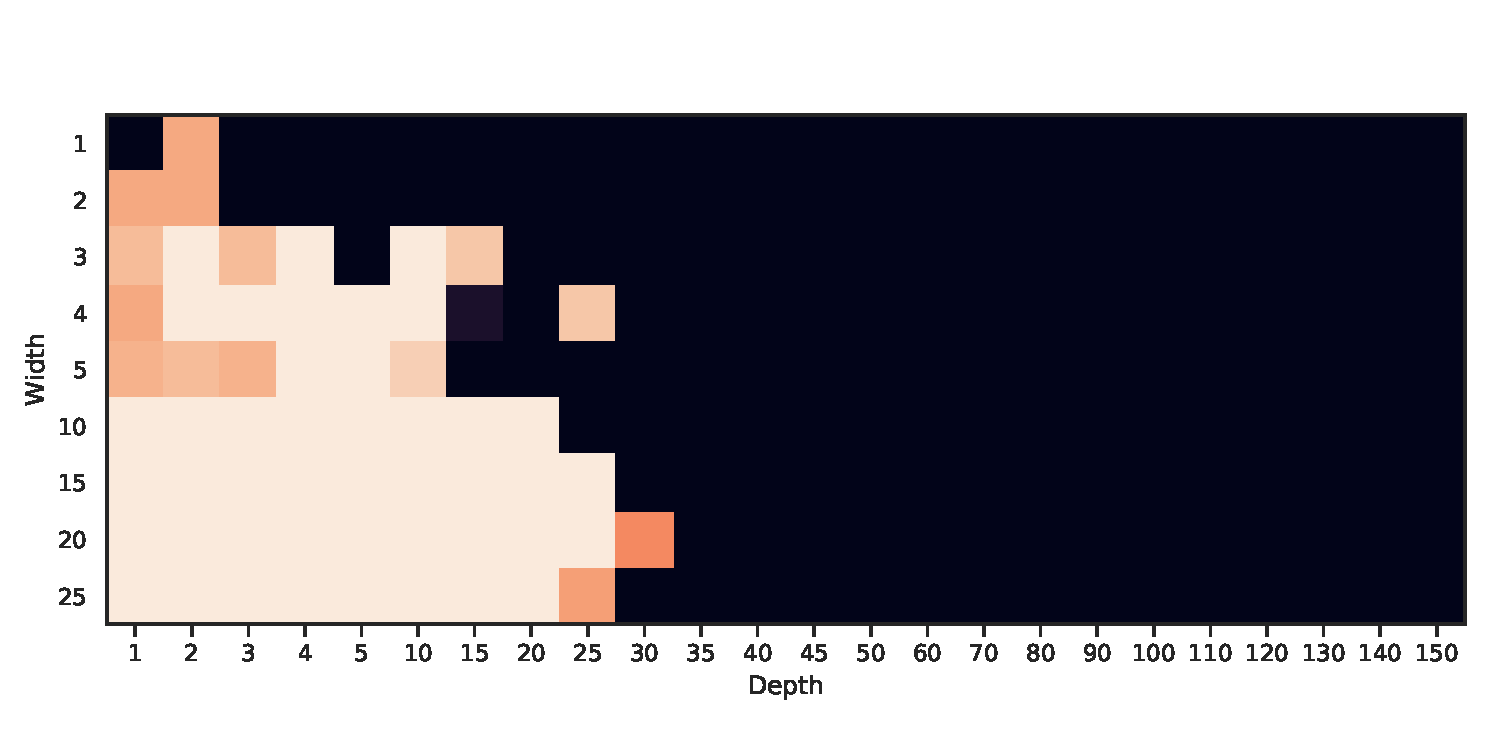
\includegraphics[width=\textwidth]{img/moons_grid/acc-relu.pdf}
        \caption{\ReLU}
        \label{fig:moons_grid_relu}
    \end{subfigure}
    ~ %add desired spacing between images, e. g. ~, \quad, \qquad, \hfill etc. 
      %(or a blank line to force the subfigure onto a new line)
    \centering
    \begin{subfigure}[b]{0.3\textwidth}
        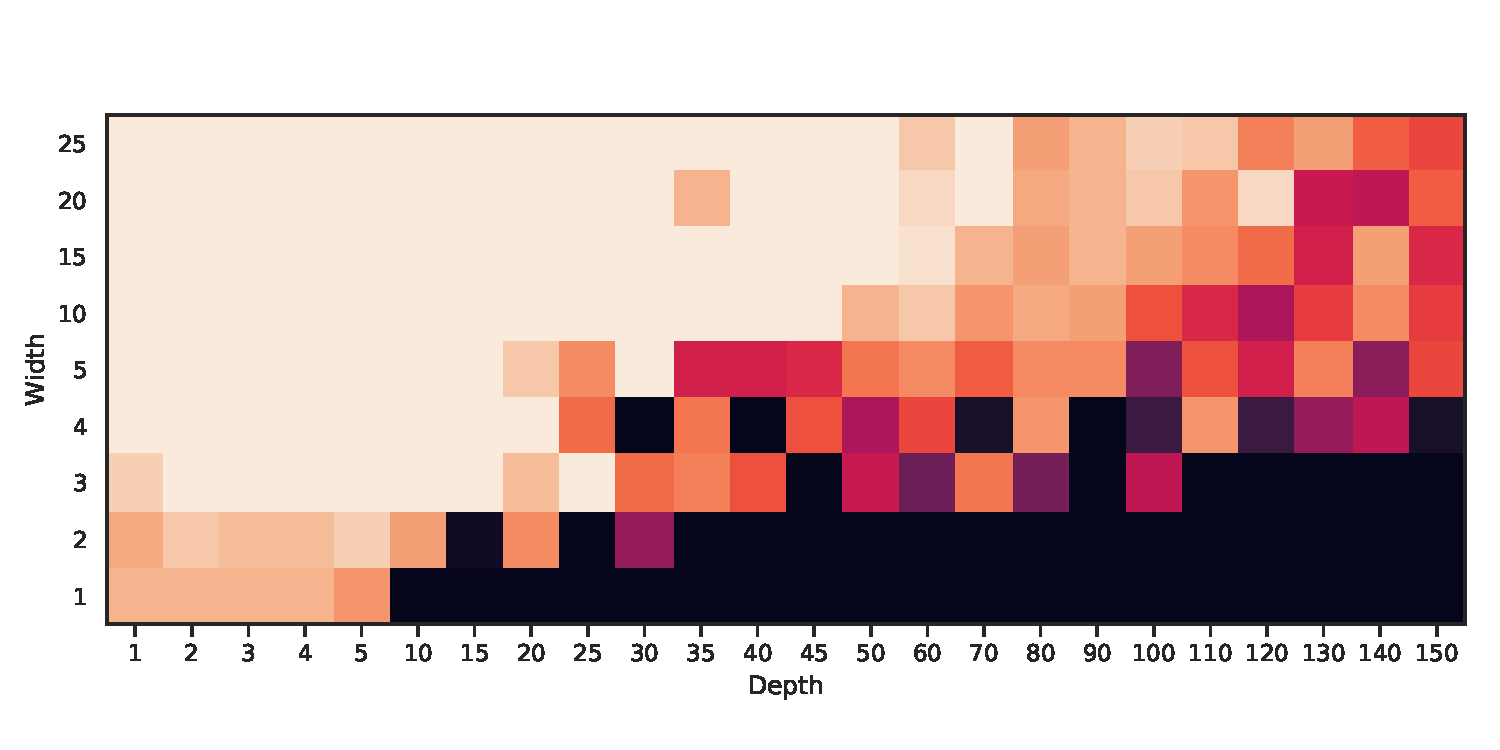
\includegraphics[width=\textwidth]{img/moons_grid/acc-relu-bn.pdf}
        \caption{\ReLUBN}
        \label{fig:moons_grid_relubn}
    \end{subfigure}
    ~ %add desired spacing between images, e. g. ~, \quad, \qquad, \hfill etc. 
      %(or a blank line to force the subfigure onto a new line)
    \centering
    \begin{subfigure}[b]{0.3\textwidth}
        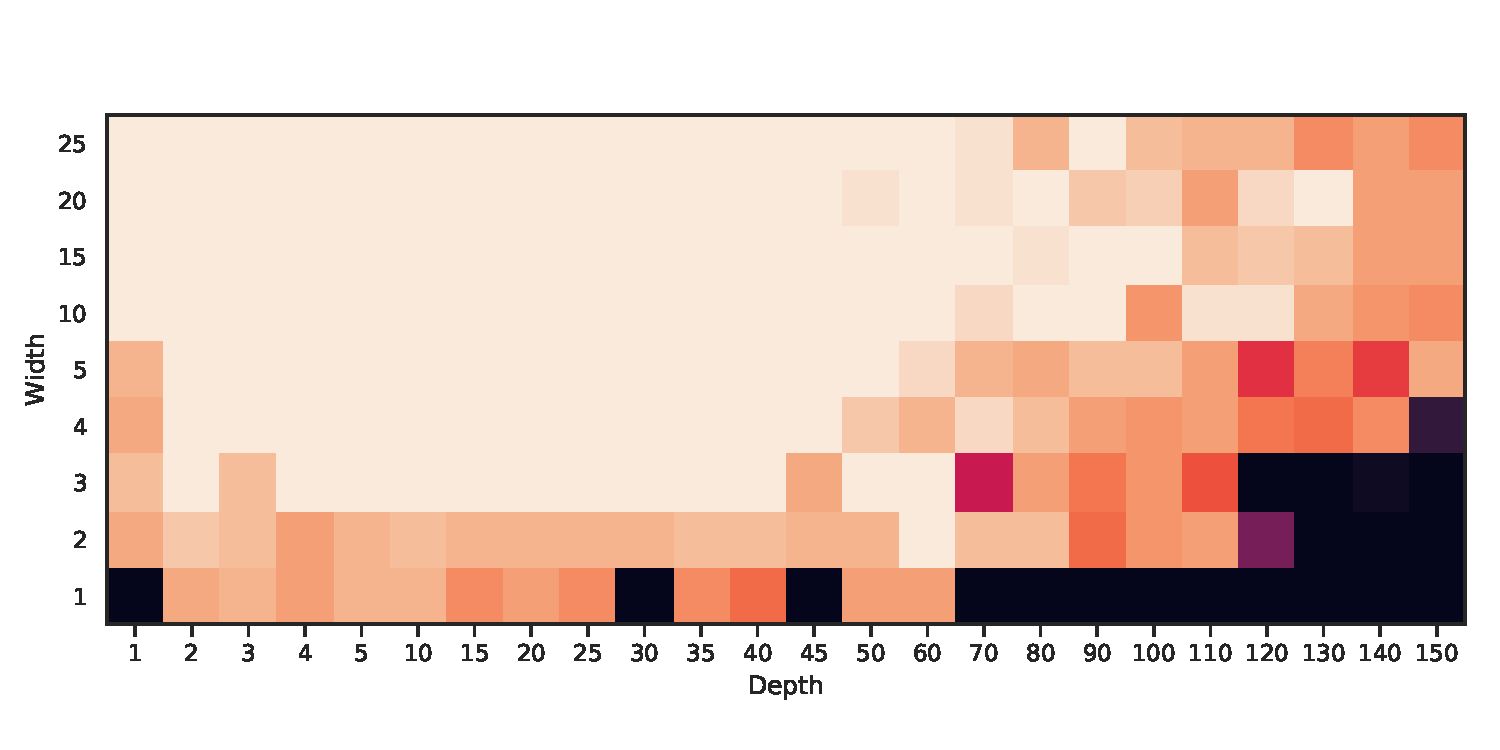
\includegraphics[width=\textwidth]{img/moons_grid/acc-sep-up-0-0001.pdf}
        \caption{\SepUnitPoint}
        \label{fig:moons_grid_up}
    \end{subfigure}
    ~ %add desired spacing between images, e. g. ~, \quad, \qquad, \hfill etc. 
      %(or a blank line to force the subfigure onto a new line)
    \\
    \begin{subfigure}[b]{0.3\textwidth}
        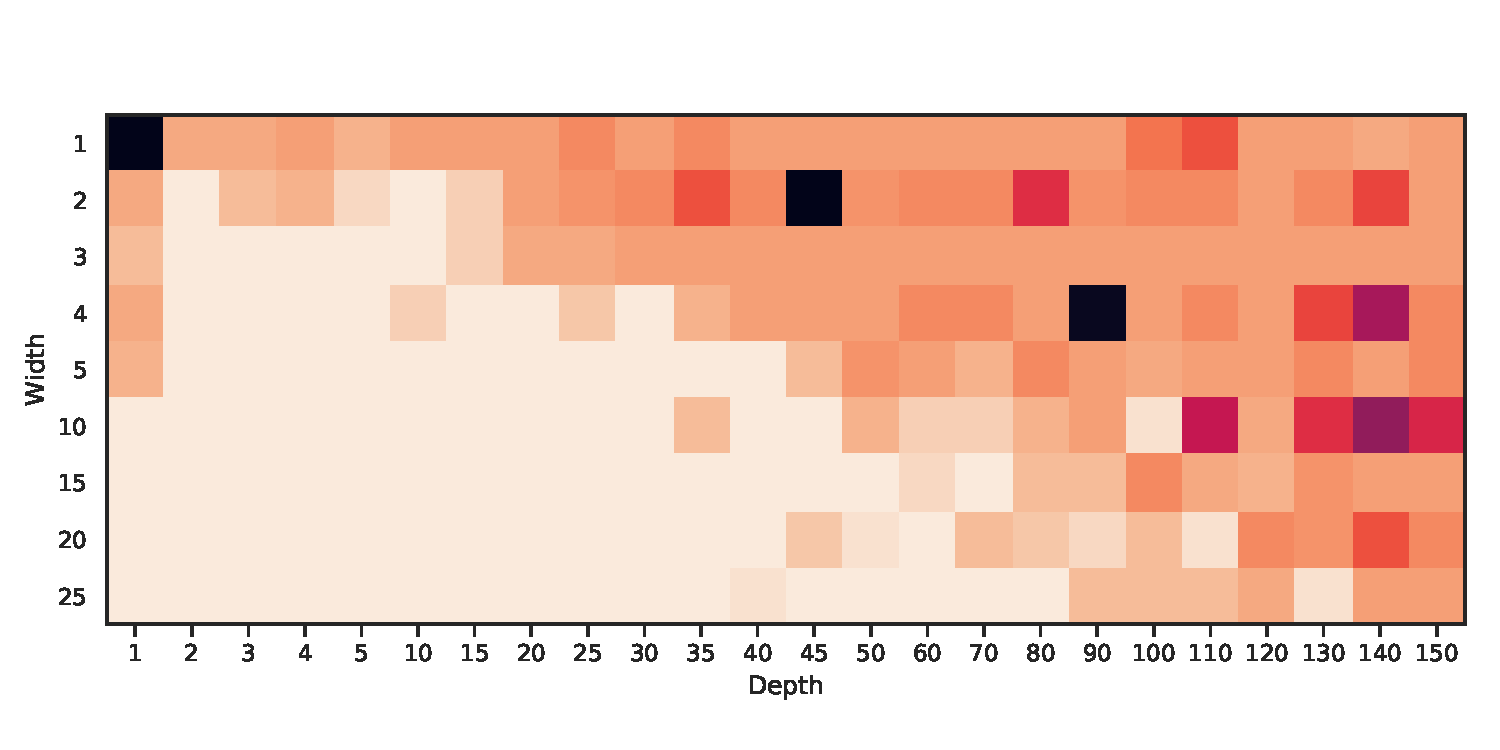
\includegraphics[width=\textwidth]{img/moons_grid/acc-sep-u-0-0001.pdf}
        \caption{\SepUnit}
        \label{fig:moons_grid_u}
    \end{subfigure}
    ~ %add desired spacing between images, e. g. ~, \quad, \qquad, \hfill etc. 
      %(or a blank line to force the subfigure onto a new line)
    \centering
    \begin{subfigure}[b]{0.3\textwidth}
        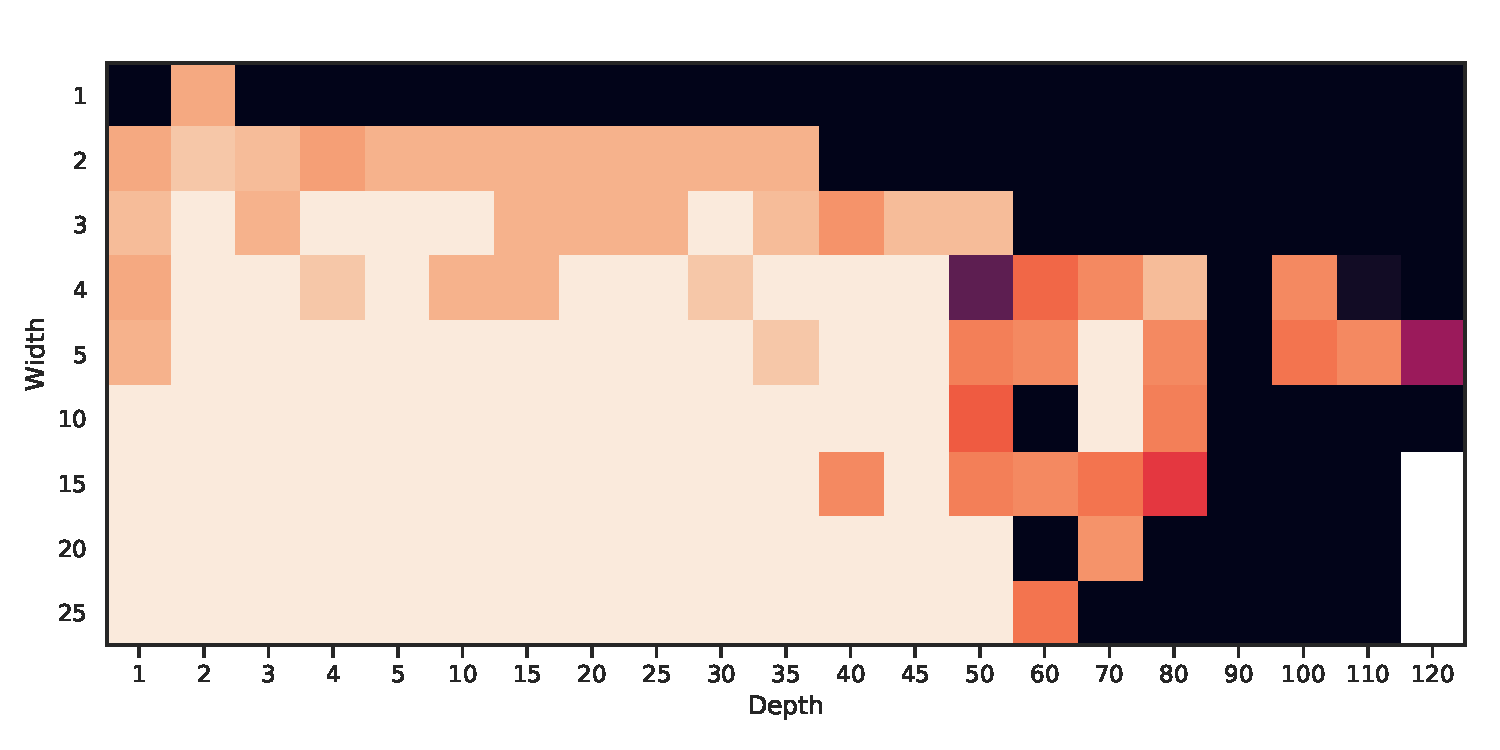
\includegraphics[width=\textwidth]{img/moons_grid/acc-sep-p-0-0001.pdf}
        \caption{\SepPoint}
        \label{fig:moons_grid_p}
    \end{subfigure}
    ~ %add desired spacing between images, e. g. ~, \quad, \qquad, \hfill etc. 
      %(or a blank line to force the subfigure onto a new line)
    \centering
    \begin{subfigure}[b]{0.3\textwidth}
        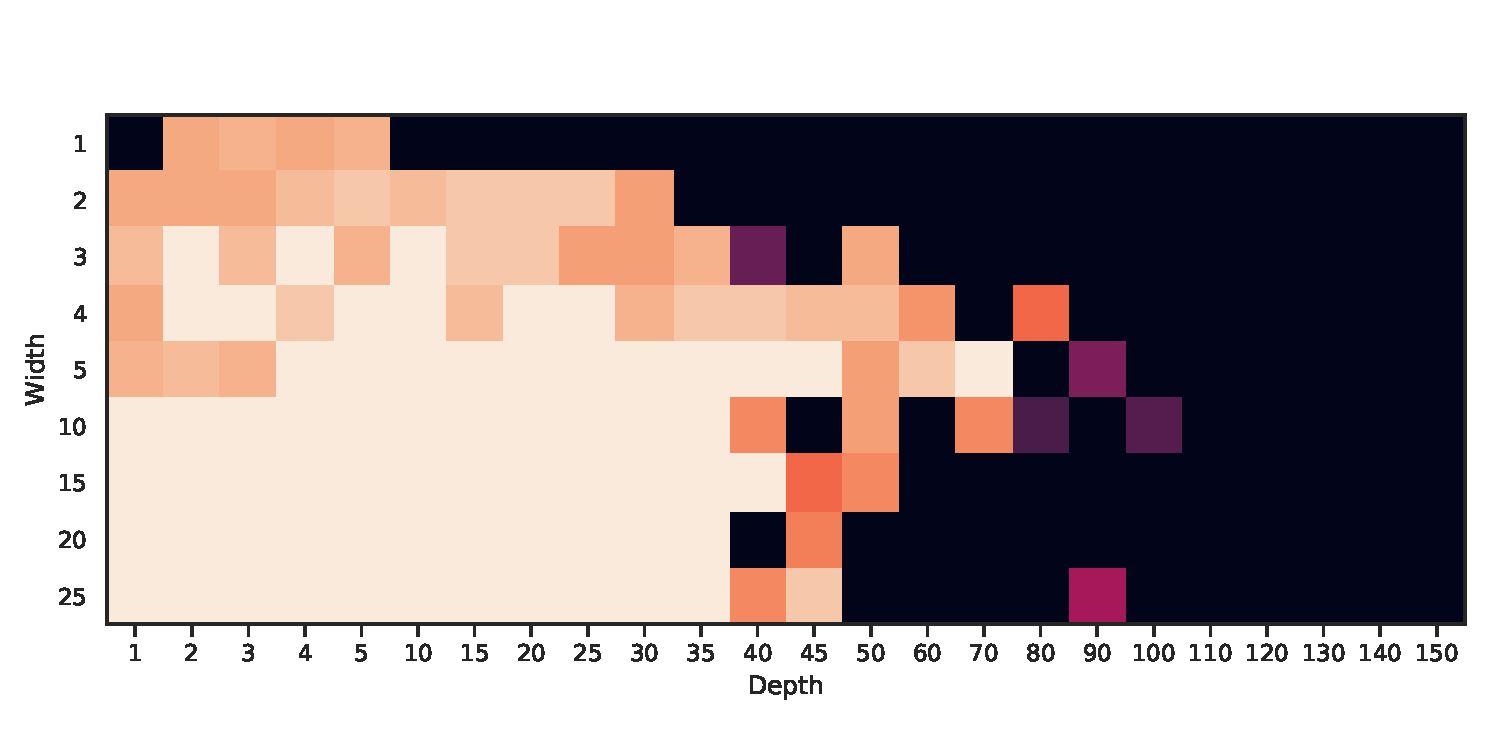
\includegraphics[width=\textwidth]{img/moons_grid/acc-sep-l-0-0001.pdf}
        \caption{\SepLayer}
        \label{fig:moons_grid_l}
    \end{subfigure}
    ~ %add desired spacing between images, e. g. ~, \quad, \qquad, \hfill etc. 
      %(or a blank line to force the subfigure onto a new line)
    
  \caption{Depth vs Width accuracy plot for a rectangular network of depth $W$ and depth $D$ varying both parameters: $2\leq W\leq 25$ and $2\leq D\leq 150$, over the \texttt{MOONS} dataset. This network were trained using an Adam scheme, and learning rate of $\gamma = 0.01$. The color map varies according to accuracy attained of each of the combinations of $W$ and $D$ (black is trivial accuracy and light cream is $1.0$)} 
  \label{fig:moons_grid} 
\end{figure*}
\subsection{On the geometry of the separation constraints}\label{subsec:geometryOfSeparation}

\begin{figure*}[h!]
  \centering
  \parbox{\textwidth}{
    \parbox{.195\textwidth}{%
      \subcaptionbox{Input layer\label{fig:moonsReLUInput}}{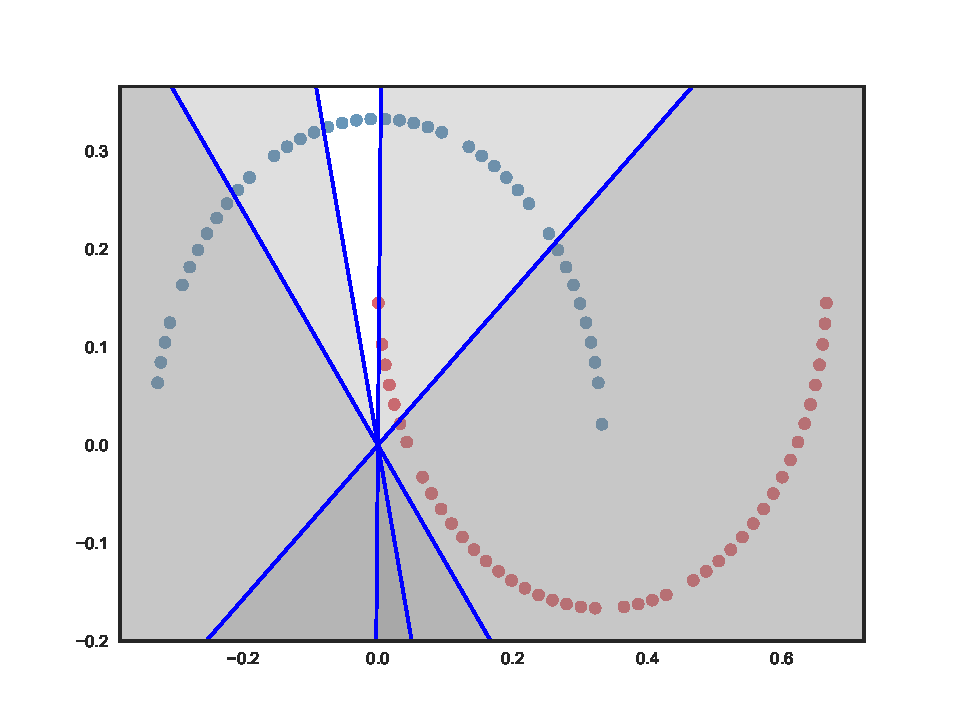
\includegraphics[width=\hsize]{img/toy/relu/conv2d_1-0.pdf}}
    }
    % \hskip1em
    \parbox{.195\textwidth}{%
      \subcaptionbox{4th layer\label{fig:moonsReLU41}}{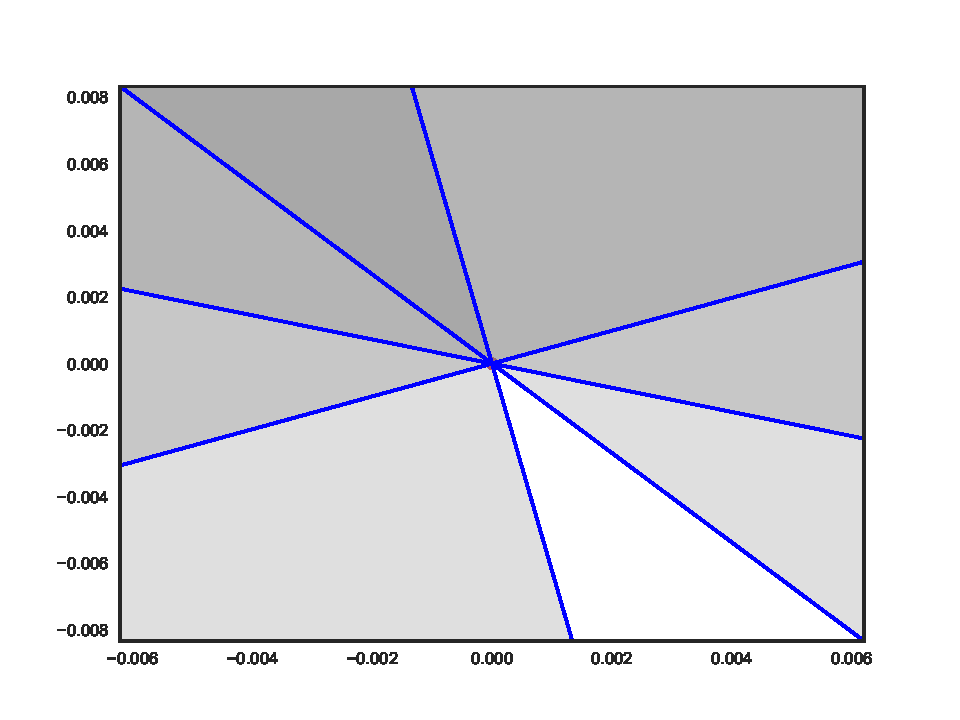
\includegraphics[width=\hsize]{img/toy/relu/conv2d_4-0.pdf}}
    %   \vskip1em
      \subcaptionbox{4th layer\label{fig:moonsReLU42}}{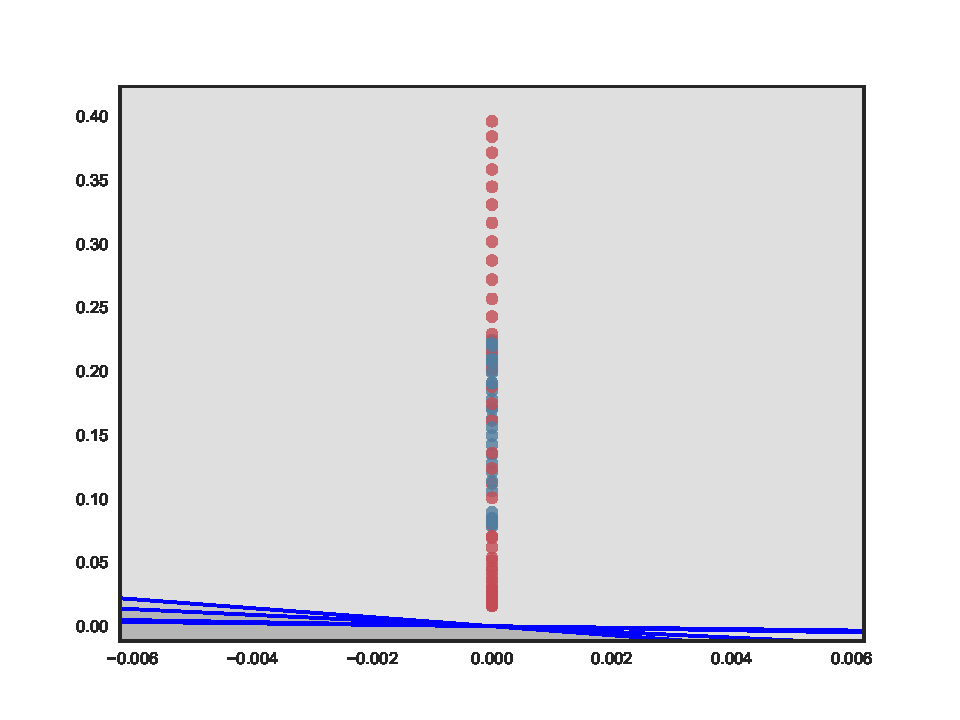
\includegraphics[width=\hsize]{img/toy/relu/conv2d_4-2.pdf}}
    }
    % \hskip1em
    \parbox{.195\textwidth}{%
      \subcaptionbox{25th layer\label{fig:moonsReLU251}}{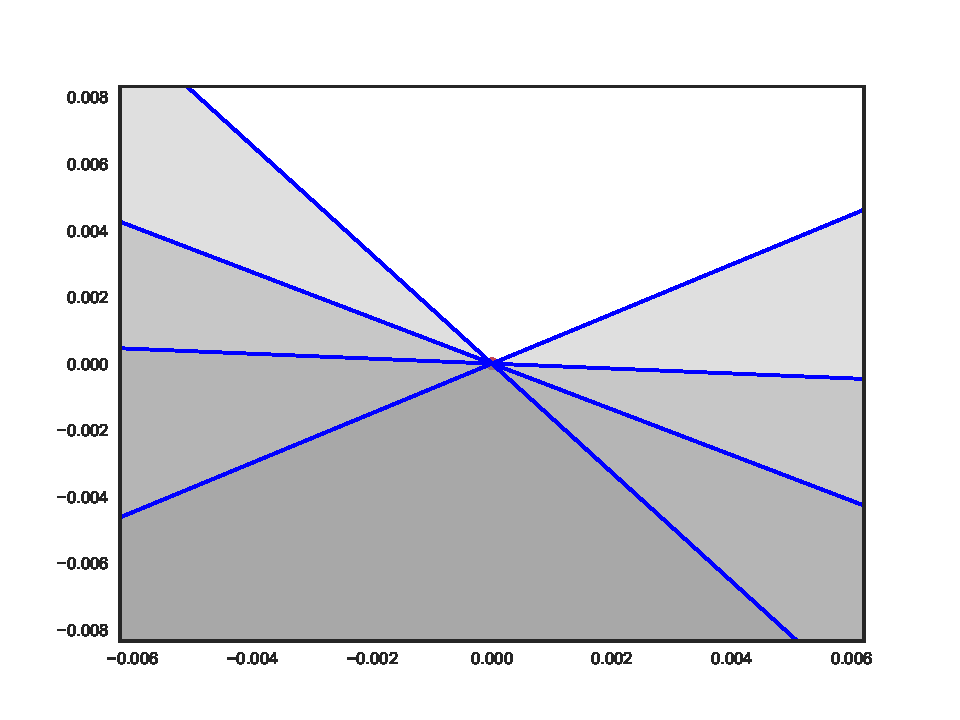
\includegraphics[width=\hsize]{img/toy/relu/conv2d_25-0.pdf}}
    %   \vskip1em
      \subcaptionbox{25th layer\label{fig:moonsReLU252}}{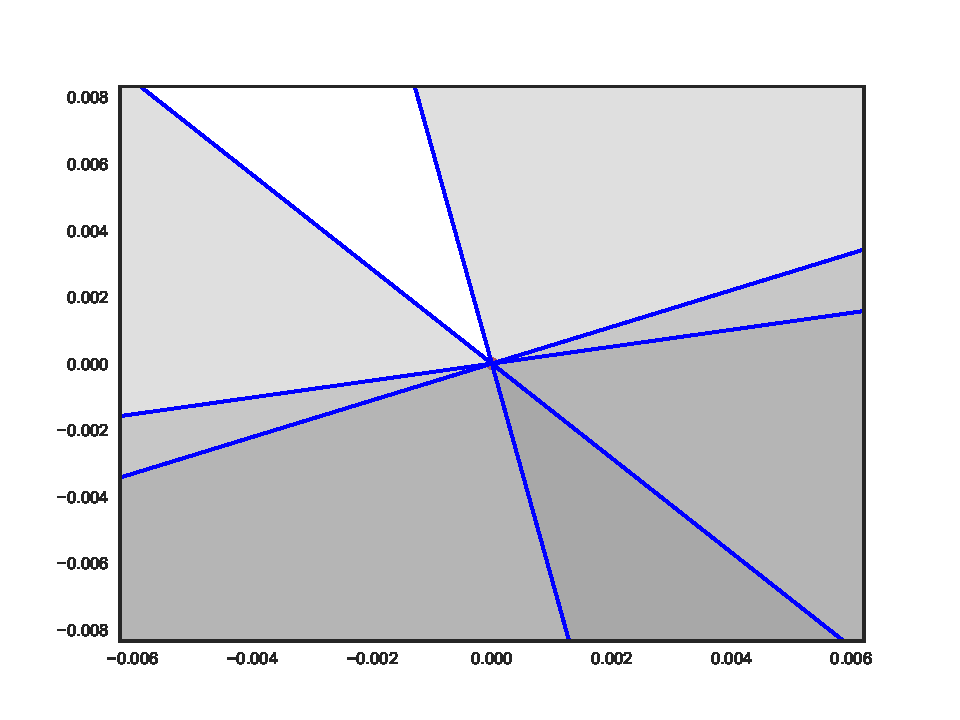
\includegraphics[width=\hsize]{img/toy/relu/conv2d_25-2.pdf}}
    }
    % \hskip1em
    \parbox{.195\textwidth}{%
      \subcaptionbox{Feature layer\label{fig:moonsReLUFeature1}}{\includegraphics[width=\hsize]{img/toy/relu/dense_1-0.pdf}}
    %   \vskip1em
      \subcaptionbox{Feature layer\label{fig:moonsReLUFeature2}}{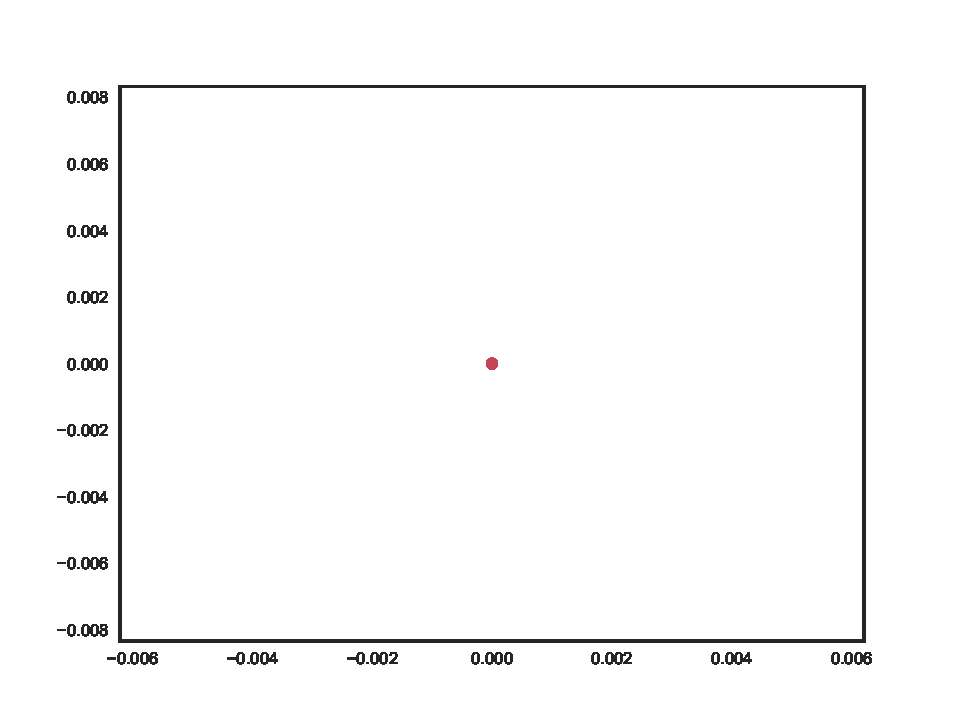
\includegraphics[width=\hsize]{img/toy/relu/dense_1-2.pdf}}
    }
    % \hskip1em
    \parbox{.195\textwidth}{%
      \subcaptionbox{Output\label{fig:moonsReLUOutput}}{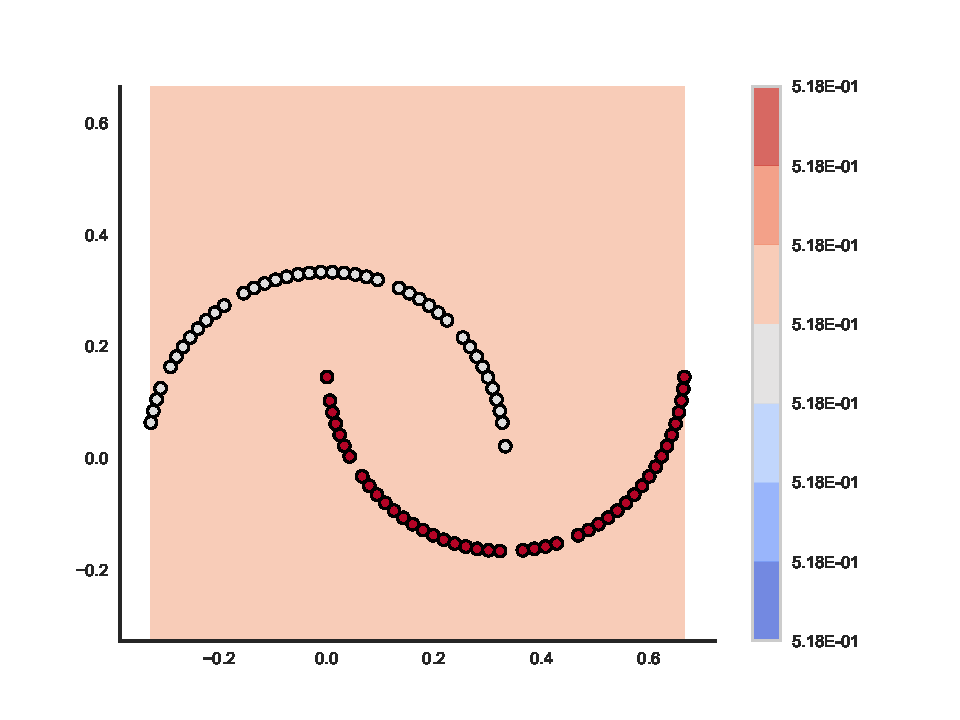
\includegraphics[clip, trim=2.35cm 1.75cm 4.5cm 0cm,width=\hsize]{img/toy/relu/output.pdf}}
    }
  }
  \caption{Data transformed across a 50x4 \ReLU classification network. Notice how the the dataset is progressively mapped to zero as it traverses the network. This renders the output layer unable to solve the problem.}
    \label{fig:moonsReLU}
\end{figure*}

\begin{figure*}[h!]
  \centering
  \parbox{\textwidth}{
    \parbox{.195\textwidth}{%
      \subcaptionbox{Input layer\label{fig:moonsReLUBNInput}}{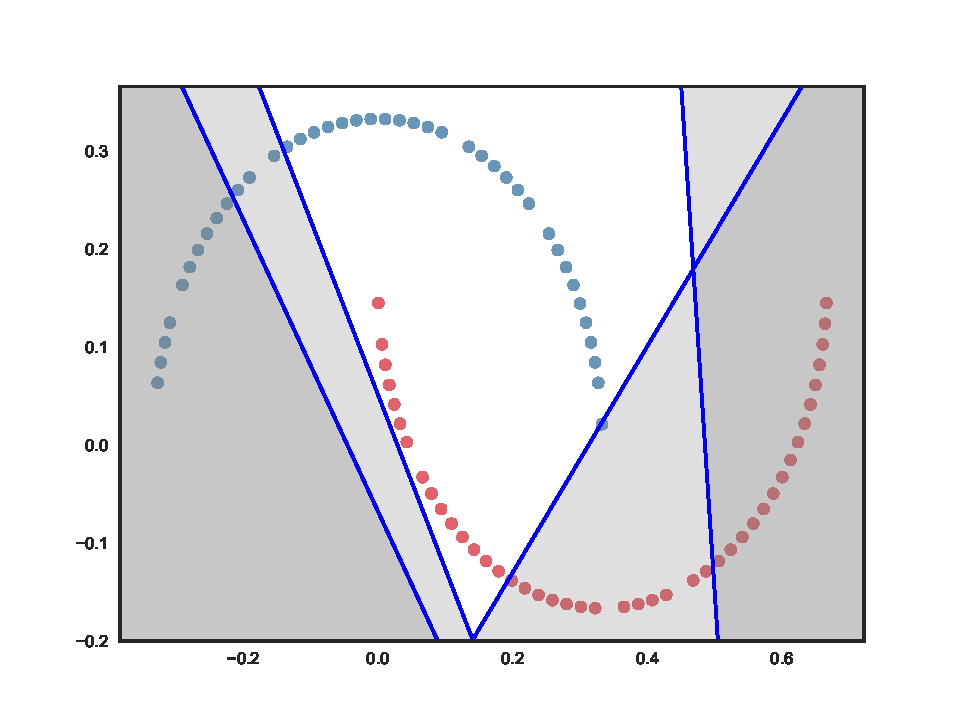
\includegraphics[width=\hsize]{img/toy/relu-bn/conv2d_1-0.pdf}}
    }
    % \hskip1em
    \parbox{.195\textwidth}{%
      \subcaptionbox{4th layer\label{fig:moonsReLUBN41}}{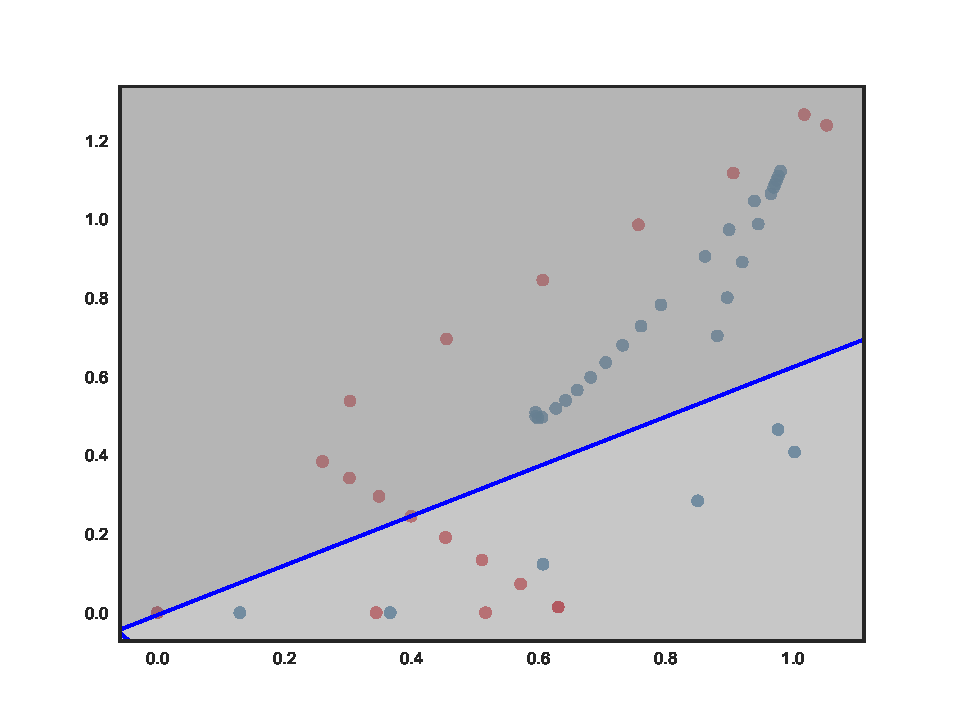
\includegraphics[width=\hsize]{img/toy/relu-bn/conv2d_4-0.pdf}}
    %   \vskip1em
      \subcaptionbox{4th layer\label{fig:moonsReLUBN42}}{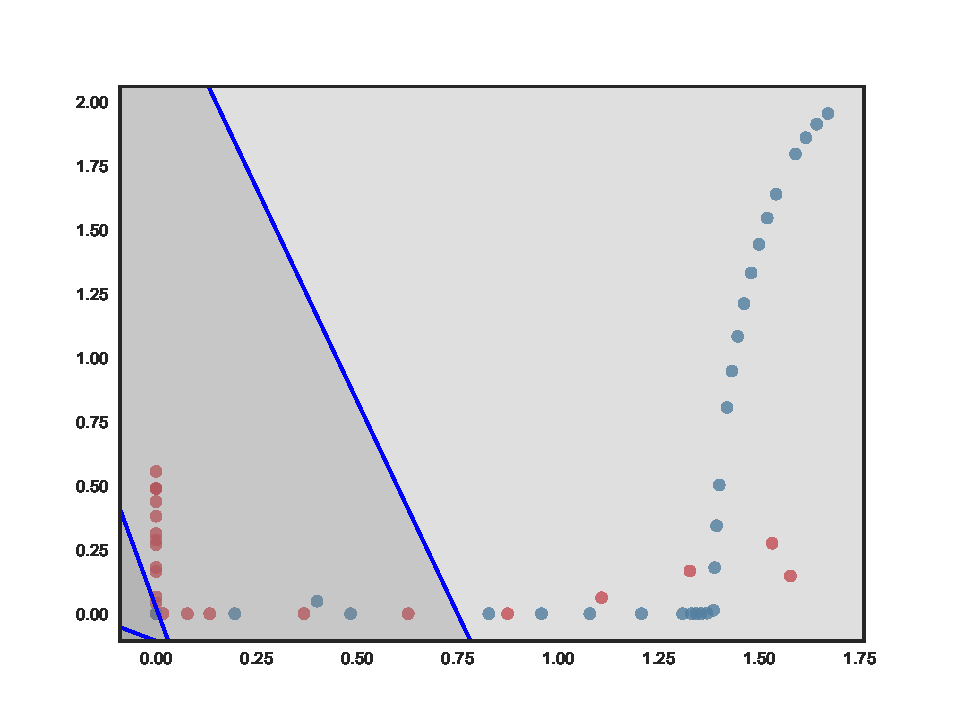
\includegraphics[width=\hsize]{img/toy/relu-bn/conv2d_4-2.pdf}}
    }
    % \hskip1em
    \parbox{.195\textwidth}{%
      \subcaptionbox{25th layer\label{fig:moonsReLUBN251}}{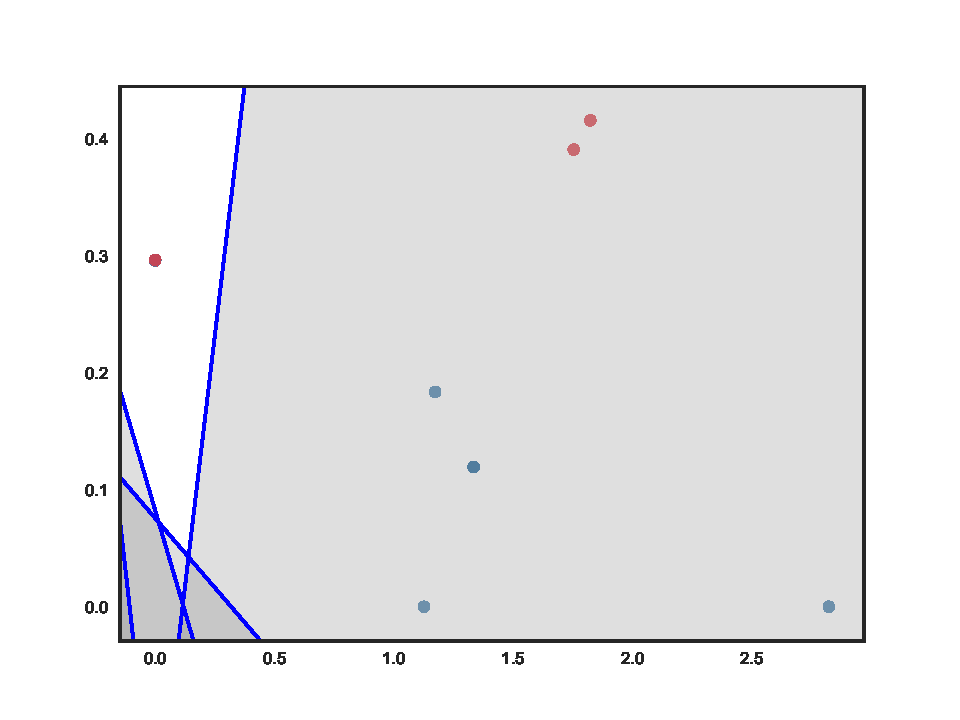
\includegraphics[width=\hsize]{img/toy/relu-bn/conv2d_25-0.pdf}}
    %   \vskip1em
      \subcaptionbox{25th layer\label{fig:moonsReLUBN252}}{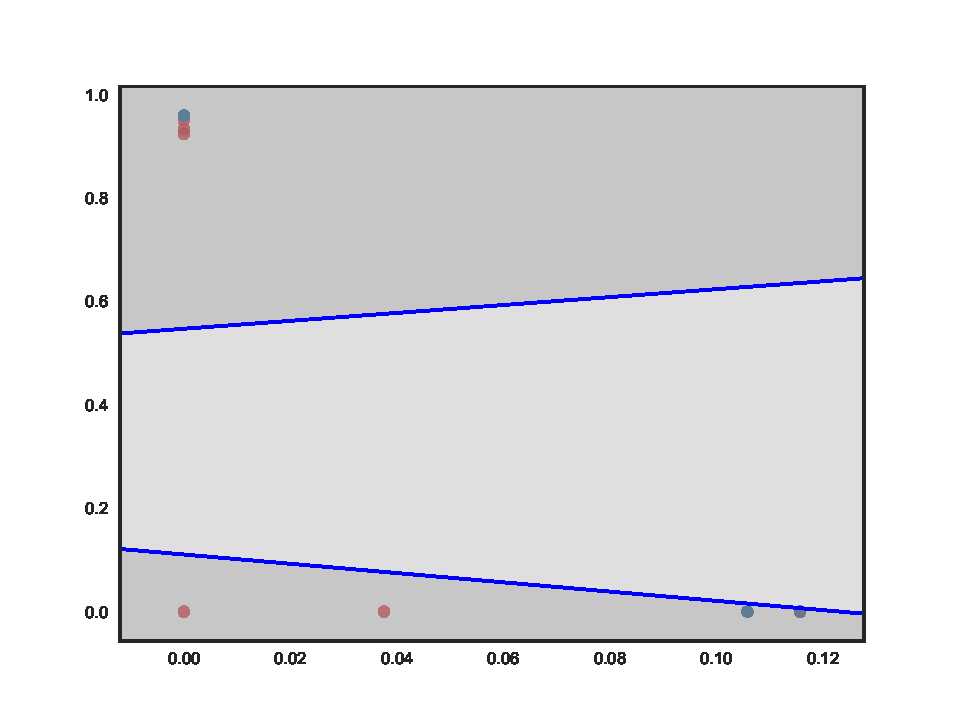
\includegraphics[width=\hsize]{img/toy/relu-bn/conv2d_25-2.pdf}} 
    }
    % \hskip1em
    \parbox{.195\textwidth}{%
      \subcaptionbox{Feature layer\label{fig:moonsReLUBNFeature1}}{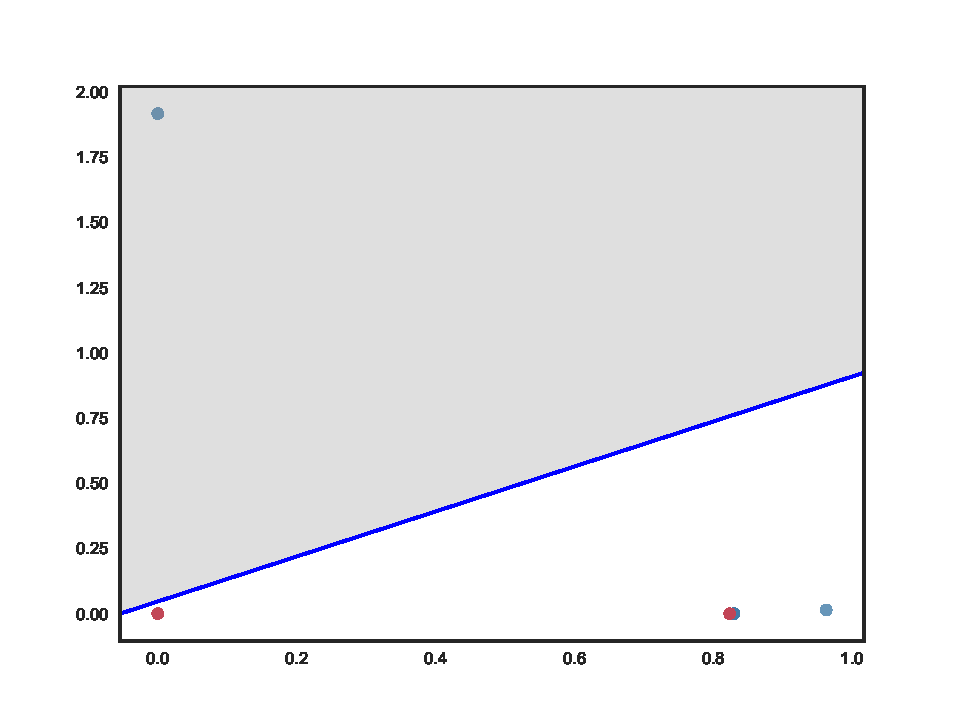
\includegraphics[width=\hsize]{img/toy/relu-bn/dense_1-0.pdf}}
    %   \vskip1em
      \subcaptionbox{Feature layer\label{fig:moonsReLUBNFeature2}}{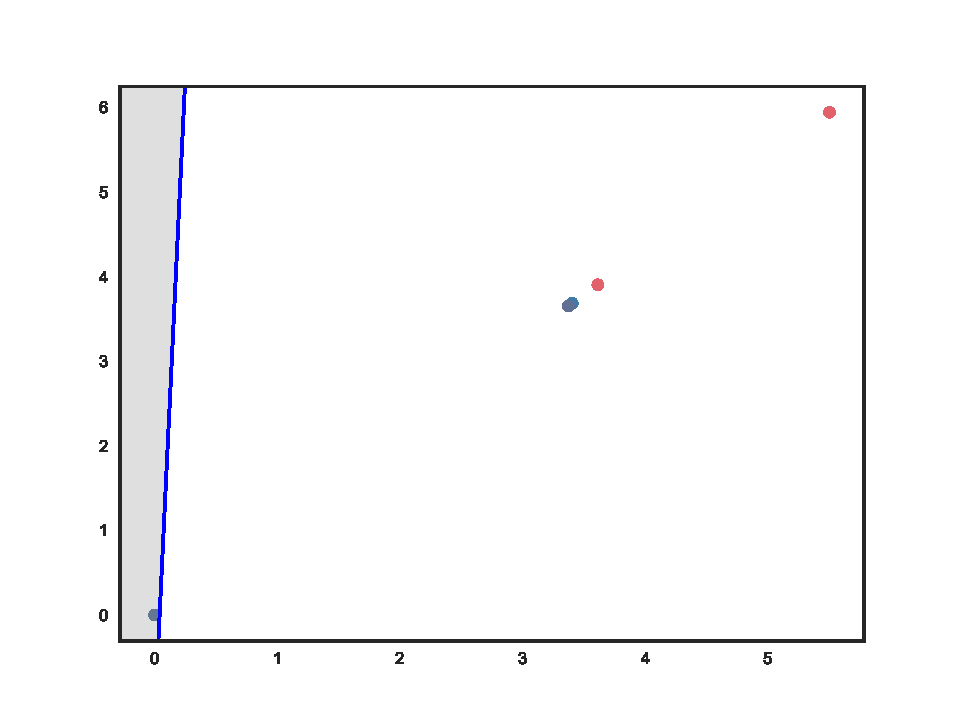
\includegraphics[width=\hsize]{img/toy/relu-bn/dense_1-2.pdf}} 
    }
    % \hskip1em
    \parbox{.195\textwidth}{%
      \subcaptionbox{Output\label{fig:moonsReLUBNOutput}}{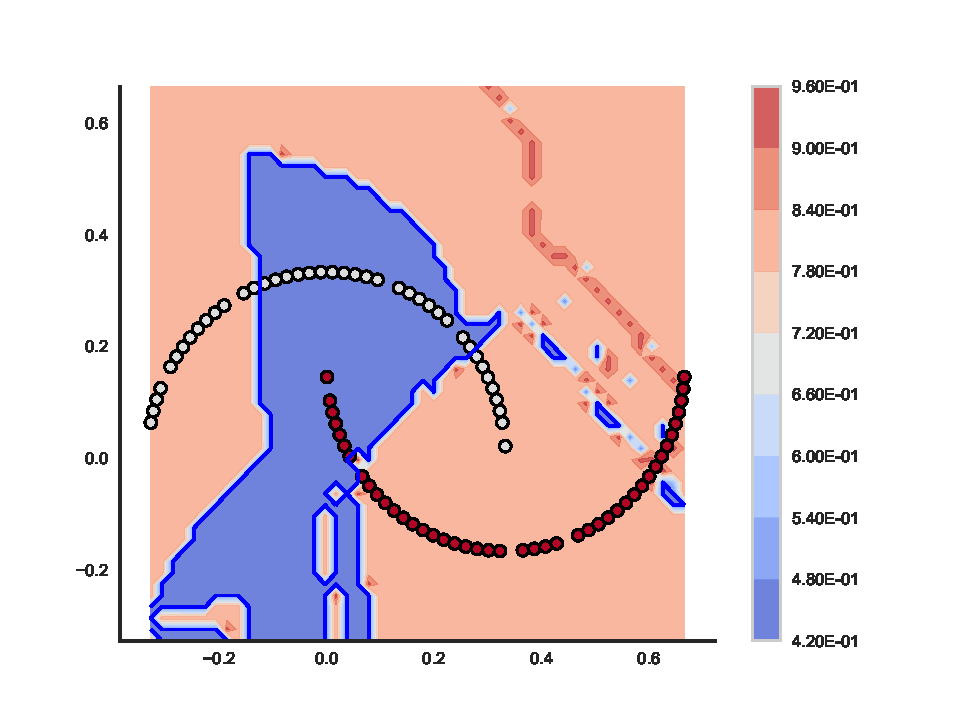
\includegraphics[clip, trim=2.35cm 1.75cm 4.5cm 0cm,width=\hsize]{img/toy/relu-bn/output.pdf}}
    }
  }
  \caption{Data transformed across a 50x4 \ReLUBN network. The dataset is collapsed in few points at the feature layer. As the gradient cannot be backpropagated across the truncation after the affine transform of $\gamma$ and $\beta$ despite the standarization, failing in the same manner than \ReLU only that with non-zero activations. This results in \emph{topological mixing} of the datasets. Therefore, the representational capability of the network is hindered to such extent that the resulting output, although non-trivial, is totally arbitrary.}
    \label{fig:moonsReLUBN}
\end{figure*}


\begin{figure*}[h!]
  \centering
     % Unitwise
  \parbox{\textwidth}{
    \parbox{.195\textwidth}{%
      \subcaptionbox{Input layer\label{fig:moonsUnitwiseInput}}{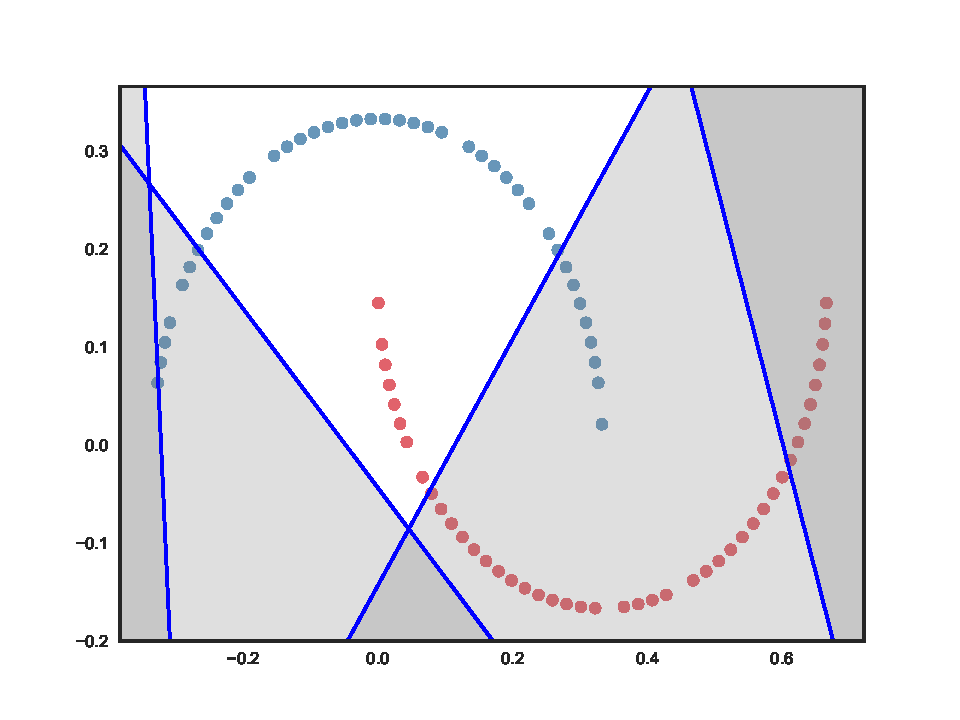
\includegraphics[width=\hsize]{img/toy/unitwise/conv2d_1-0.pdf}}
    }
    % \hskip1em
    \parbox{.195\textwidth}{%
      \subcaptionbox{4th layer\label{fig:moonsUnitwise41}}{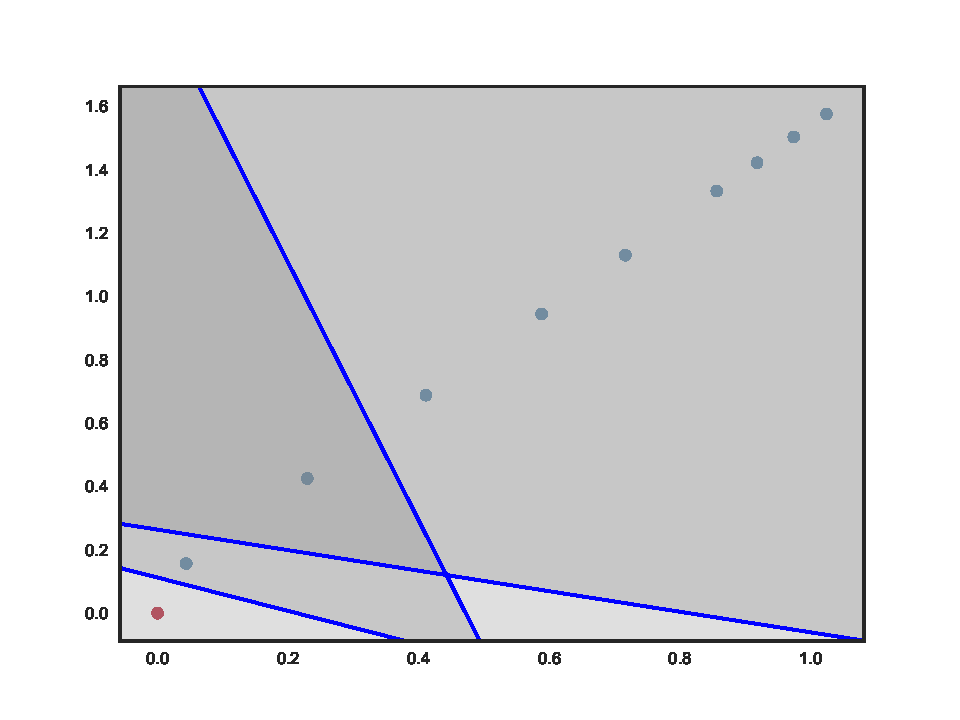
\includegraphics[width=\hsize]{img/toy/unitwise/conv2d_4-0.pdf}}
    %   \vskip1em
      \subcaptionbox{4th layer\label{fig:moonsUnitwise42}}{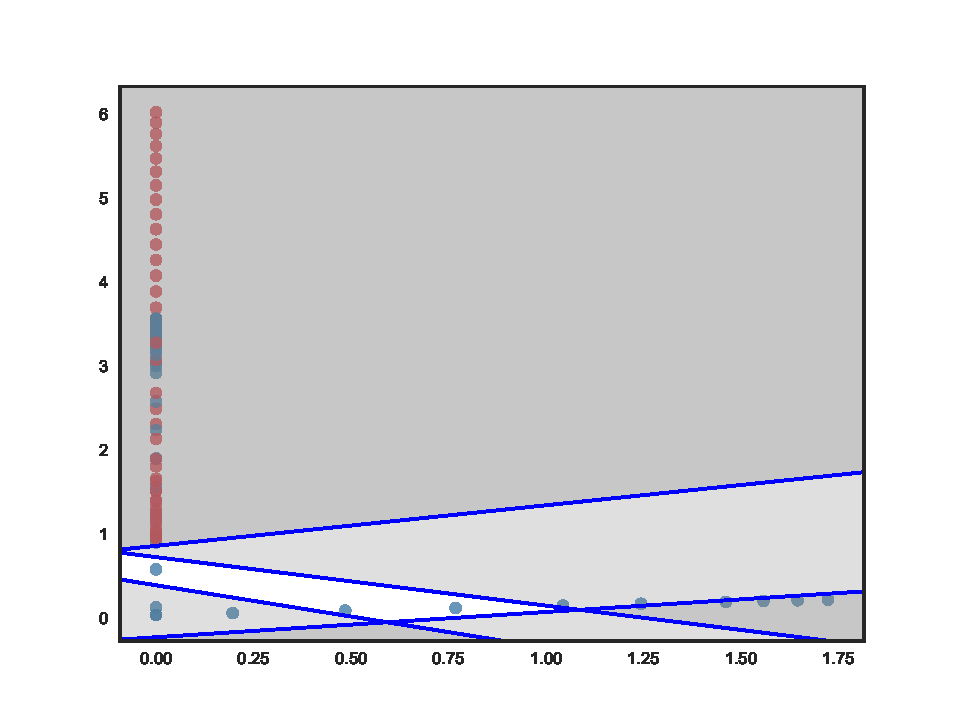
\includegraphics[width=\hsize]{img/toy/unitwise/conv2d_4-2.pdf}}
    }
    % \hskip1em
    \parbox{.195\textwidth}{%
      \subcaptionbox{25th layer\label{fig:moonsUnitwise251}}{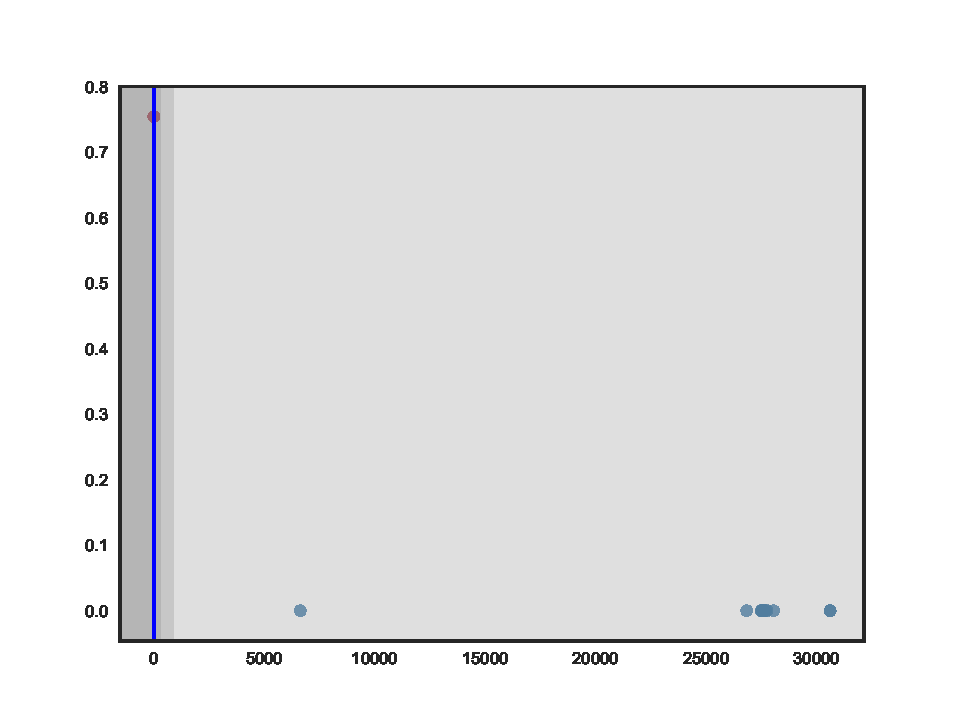
\includegraphics[width=\hsize]{img/toy/unitwise/conv2d_25-0.pdf}}
    %   \vskip1em
      \subcaptionbox{25th layer\label{fig:moonsUnitwise252}}{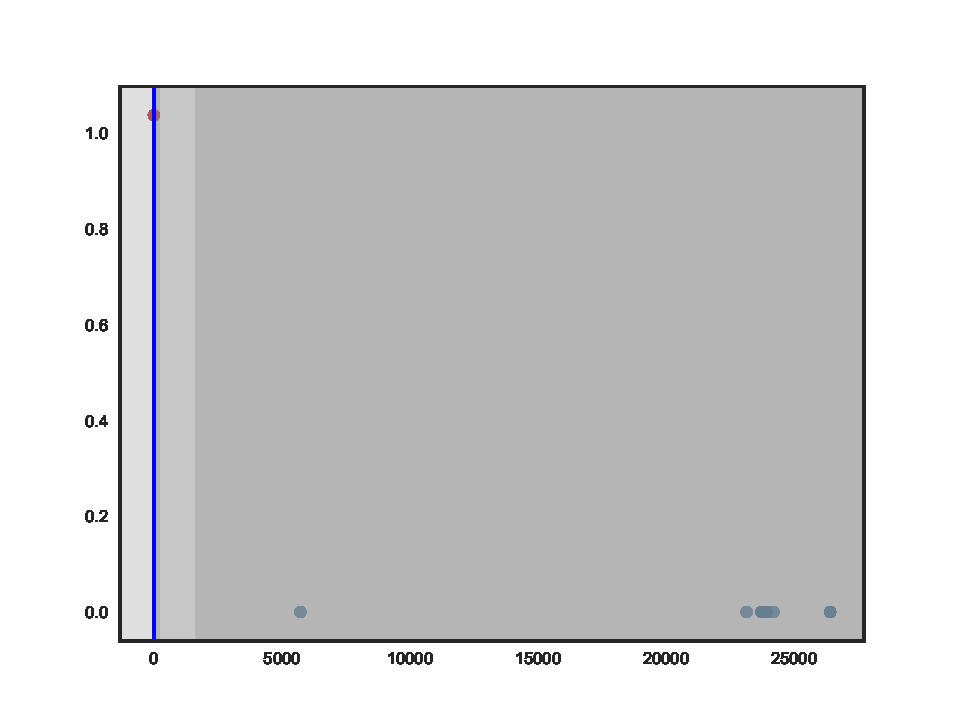
\includegraphics[width=\hsize]{img/toy/unitwise/conv2d_25-2.pdf}}
    }
    % \hskip1em
    \parbox{.195\textwidth}{%
      \subcaptionbox{Feature layer\label{fig:moonsUnitwiseFeature1}}{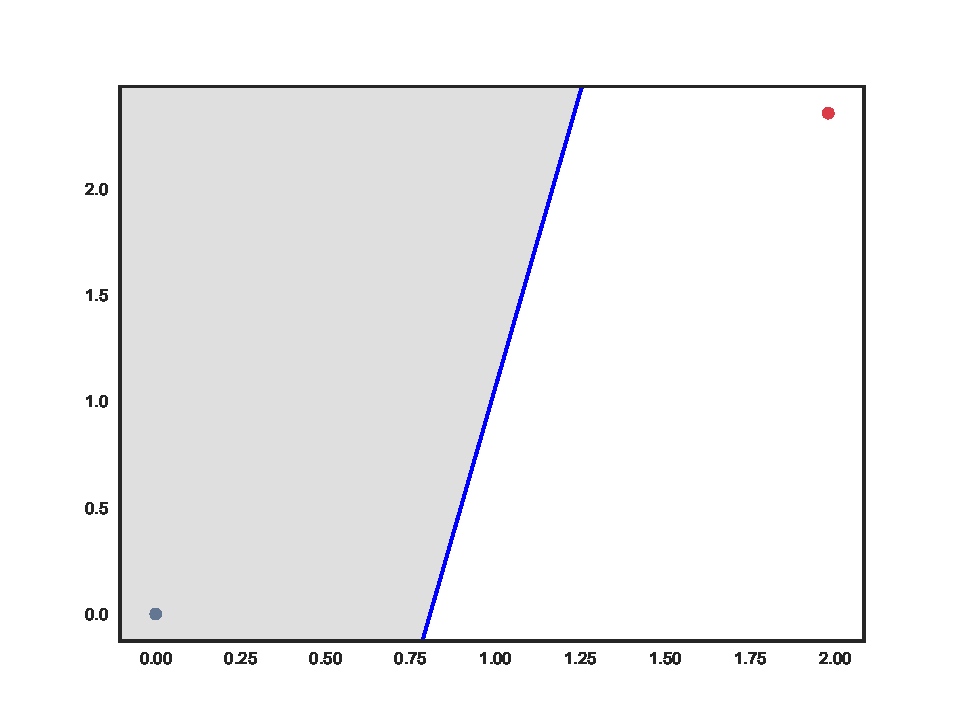
\includegraphics[width=\hsize]{img/toy/unitwise/dense_1-0.pdf}}
    %   \vskip1em
      \subcaptionbox{Feature layer\label{fig:moonsUnitwiseFeature2}}{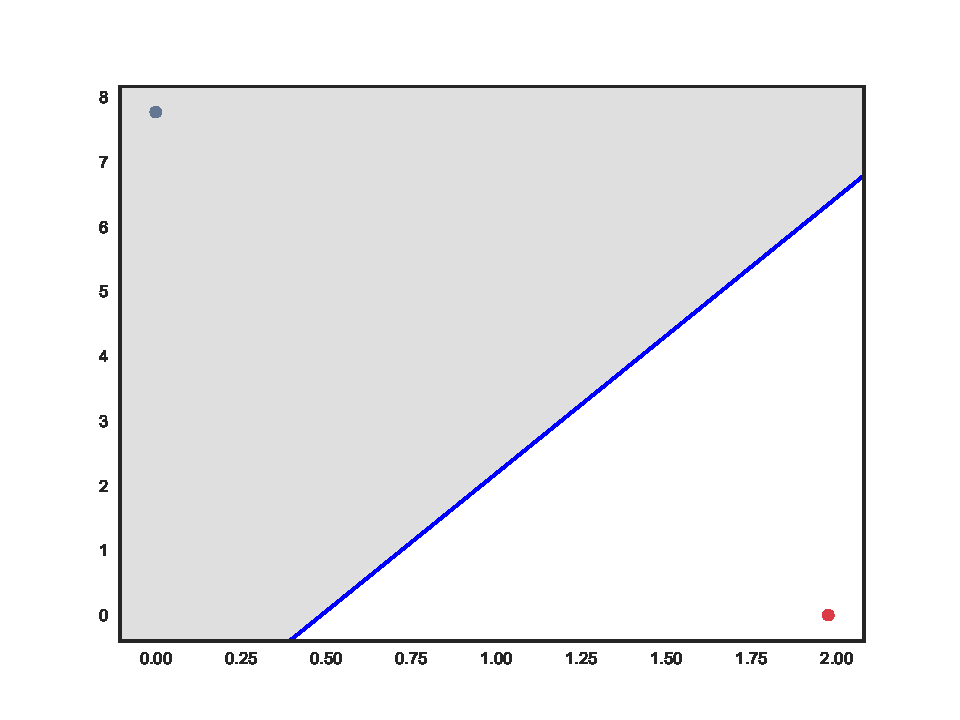
\includegraphics[width=\hsize]{img/toy/unitwise/dense_1-2.pdf}}
    }
    % \hskip1em
    \parbox{.195\textwidth}{%
      \subcaptionbox{Output\label{fig:moonsUnitwiseOutput}}{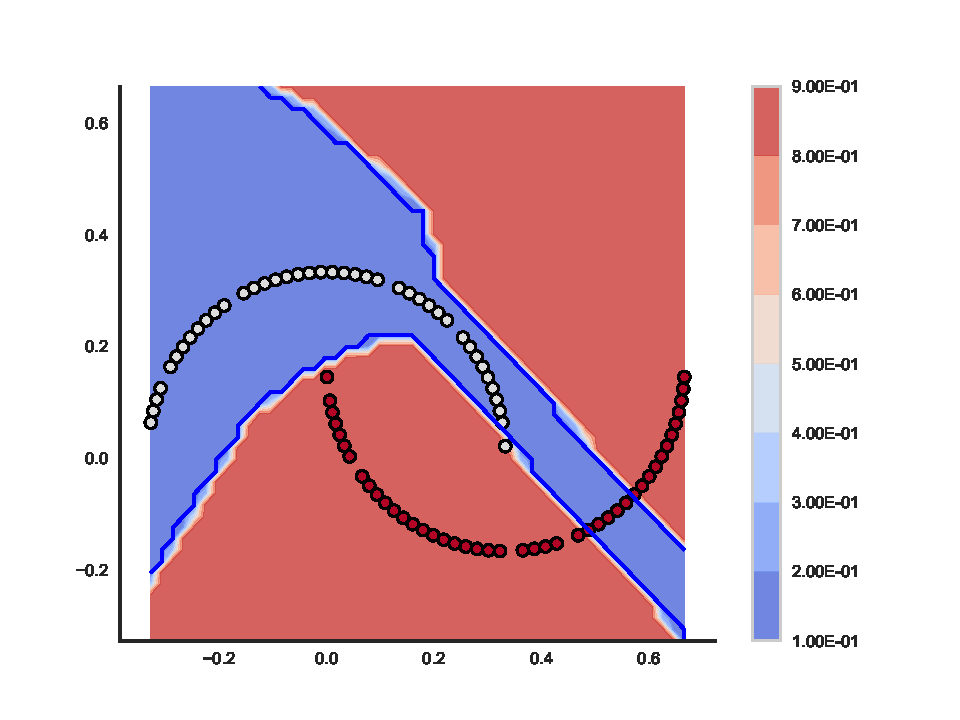
\includegraphics[clip, trim=2.35cm 1.75cm 4.5cm 0cm,width=\hsize]{img/toy/unitwise/output.pdf}}
    }
  }
  \caption{Data transformed across a 50x4 \SepUnit network. Notice how dead and affine units have been reduced. Despite collapsing the dataset in two points at the feature layer, the classification performed in the output layer is approximately correct. We conjecture that this is due the dead point addressed with \SepPoint.}
    \label{fig:moonsUnitwise}
\end{figure*}



\begin{figure*}[h!]
  \centering
  %Pointwise
  \parbox{\textwidth}{
    \parbox{.195\textwidth}{%
      \subcaptionbox{Input layer\label{fig:moonsPointwiseInput}}{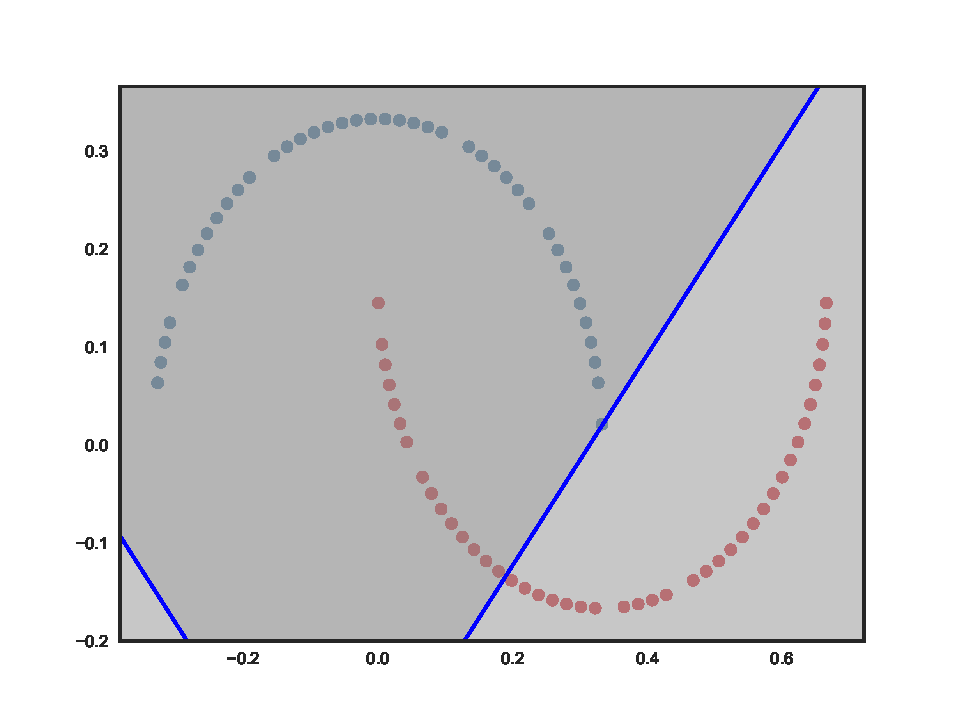
\includegraphics[width=\hsize]{img/toy/pointwise/conv2d_1-0.pdf}}
    }
    % \hskip1em
    \parbox{.195\textwidth}{%
      \subcaptionbox{4th layer\label{fig:moonsPointwise41}}{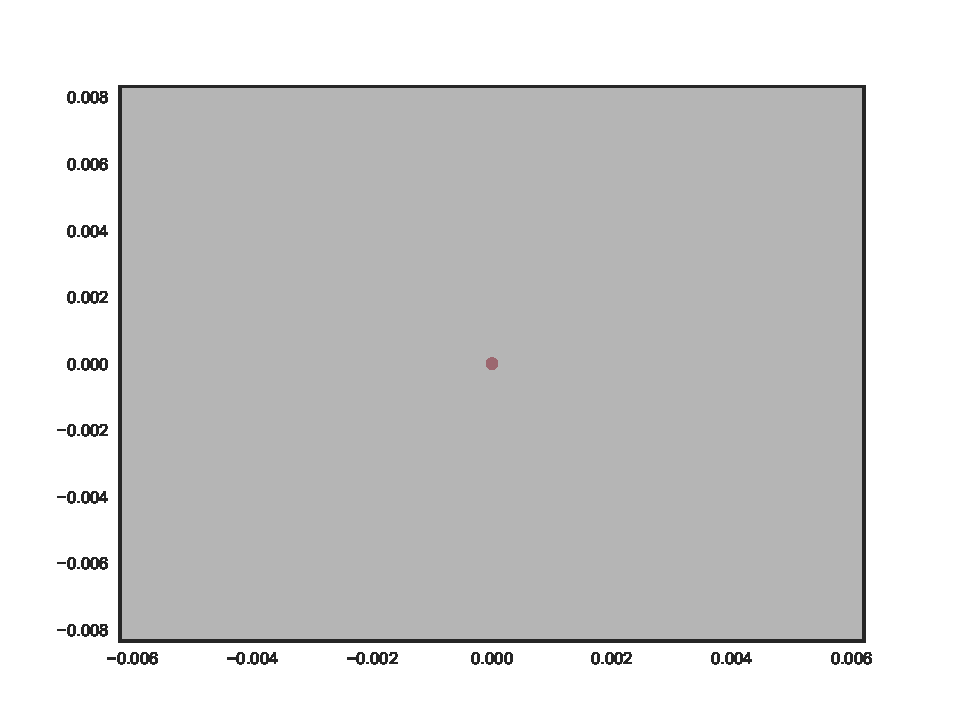
\includegraphics[width=\hsize]{img/toy/pointwise/conv2d_4-0.pdf}}
    %   \vskip1em
      \subcaptionbox{4th layer\label{fig:moonsPointwise42}}{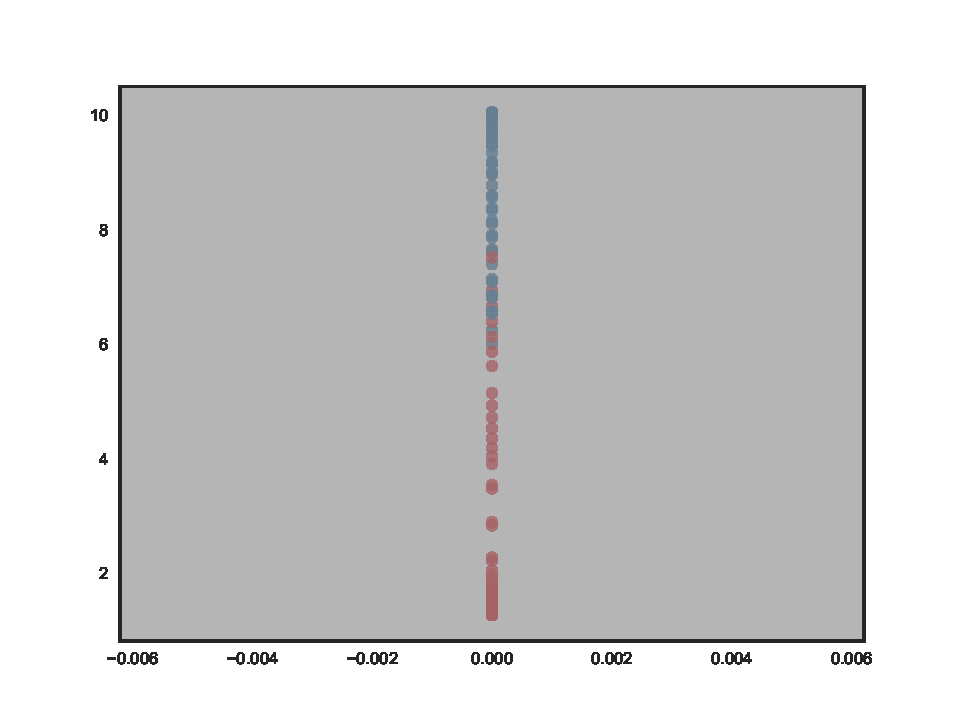
\includegraphics[width=\hsize]{img/toy/pointwise/conv2d_4-2.pdf}} 
    }
    % \hskip1em
    \parbox{.195\textwidth}{%
      \subcaptionbox{25th layer\label{fig:moonsPointwise251}}{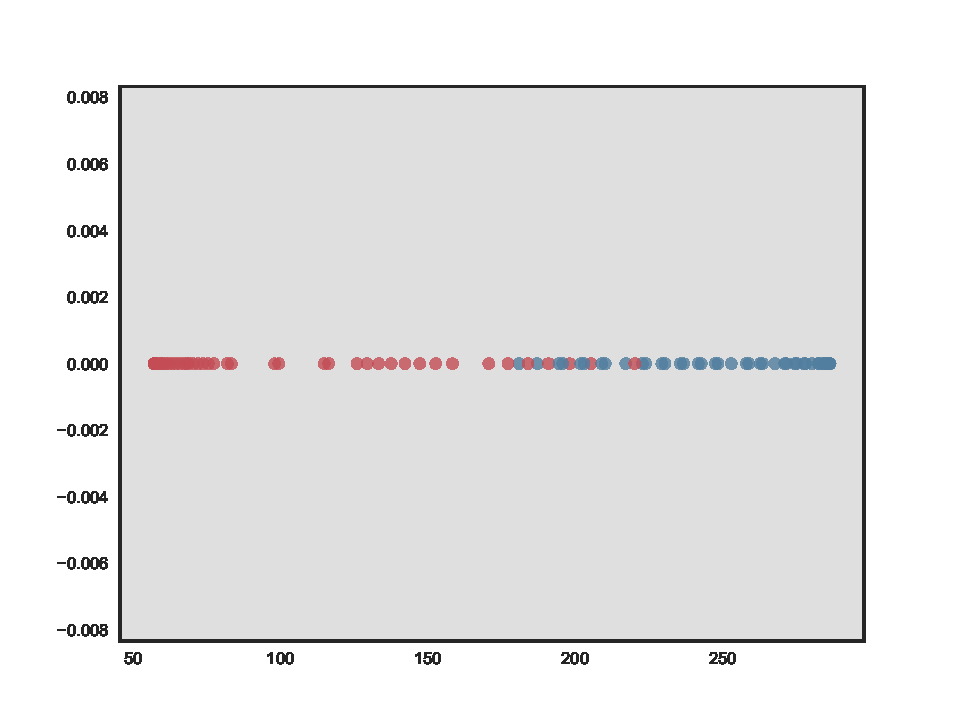
\includegraphics[width=\hsize]{img/toy/pointwise/conv2d_25-0.pdf}}
    %   \vskip1em
      \subcaptionbox{25th layer\label{fig:moonsPointwise252}}{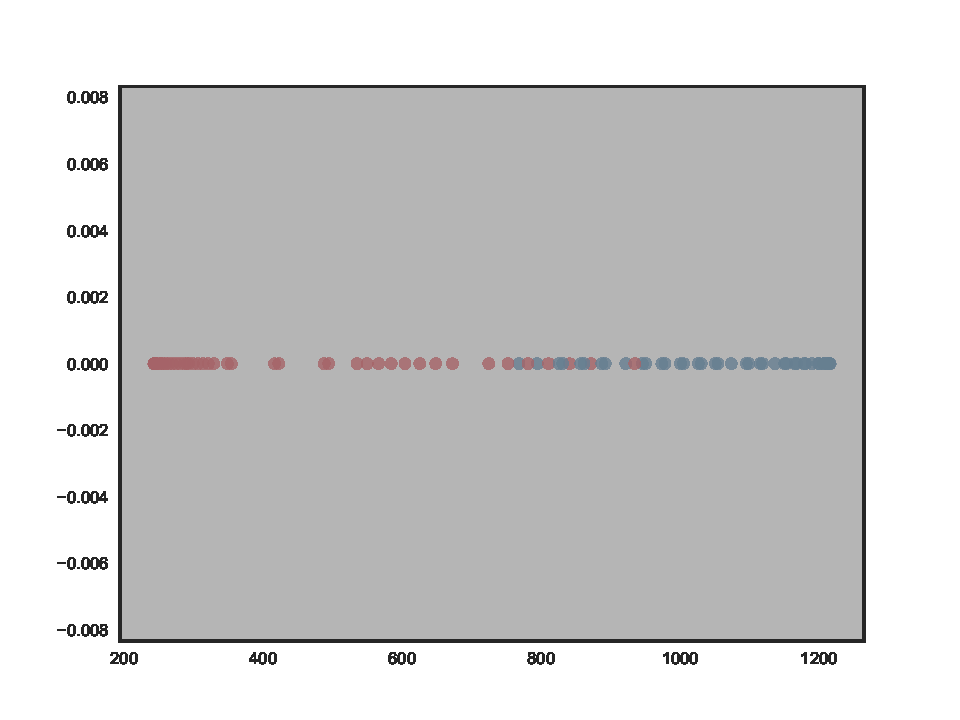
\includegraphics[width=\hsize]{img/toy/pointwise/conv2d_25-2.pdf}} 
    }
    % \hskip1em
    \parbox{.195\textwidth}{%
      \subcaptionbox{Feature layer\label{fig:moonsPointwiseFeature1}}{\includegraphics[width=\hsize]{img/toy/pointwise/dense_1-0.pdf}}
    %   \vskip1em
      \subcaptionbox{Feature layer\label{fig:moonsPointwiseFeature2}}{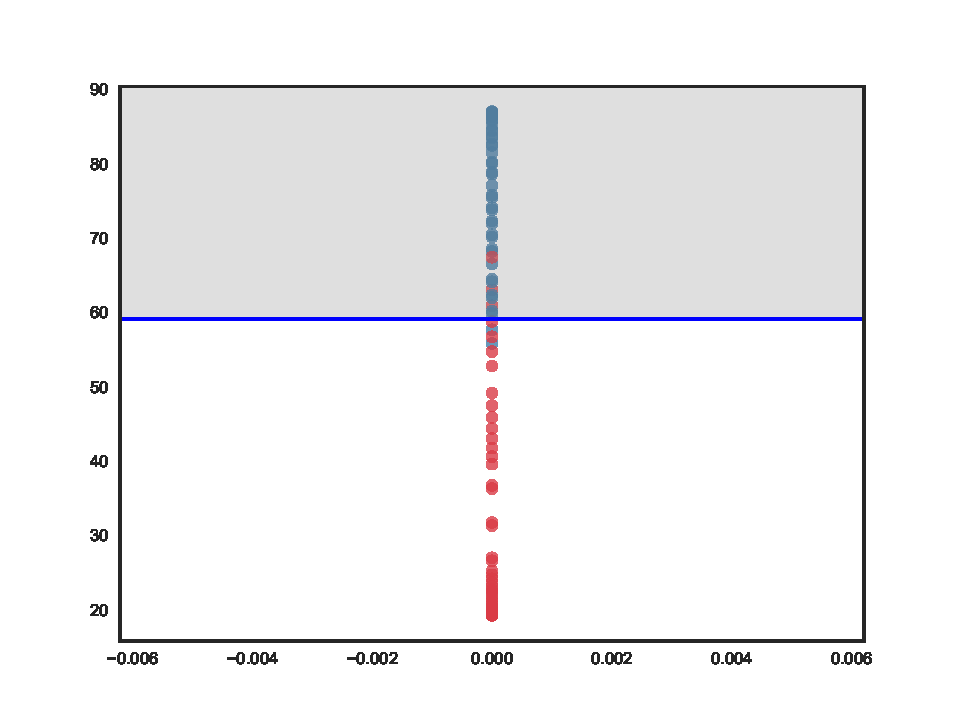
\includegraphics[width=\hsize]{img/toy/pointwise/dense_1-2.pdf}} 
    }
    % \hskip1em
    \parbox{.195\textwidth}{%
      \subcaptionbox{Output\label{fig:moonsPointwiseOutput}}{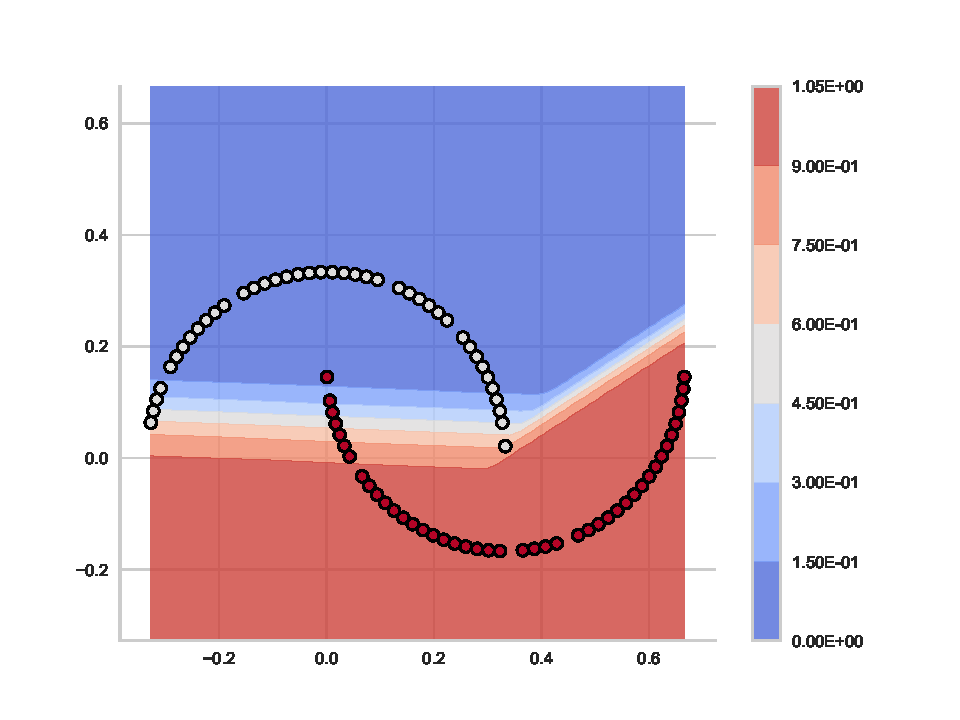
\includegraphics[clip, trim=2.35cm 1.75cm 4.5cm 0cm,width=\hsize]{img/toy/pointwise/output.pdf}}
    }
  }
  \caption{Data transformed across a 50x4 \SepPoint network. The network displays a richer internal representation without collapsing the dataset like \SepUnit or \ReLUBN. However, plenty of dead and affine units appear since they are not penalized, causing underfitting.}
    \label{fig:moonsPointwise}
\end{figure*}


\begin{figure*}[h!]
  \centering
   \parbox{\textwidth}{
    \parbox{.195\textwidth}{%
      \subcaptionbox{Input layer\label{fig:moonsUnitpointwiseInput}}{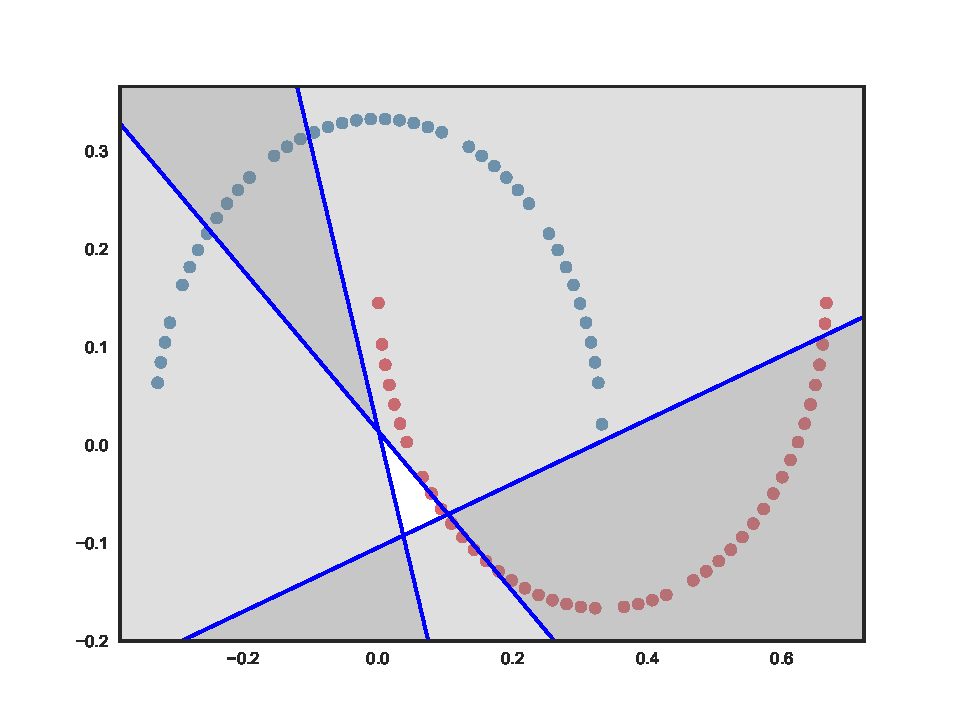
\includegraphics[width=\hsize]{img/toy/unitpointwise/conv2d_1-0.pdf}}
    }
    % \hskip1em
    \parbox{.195\textwidth}{%
      \subcaptionbox{4th layer\label{fig:moonsUnitpointwise41}}{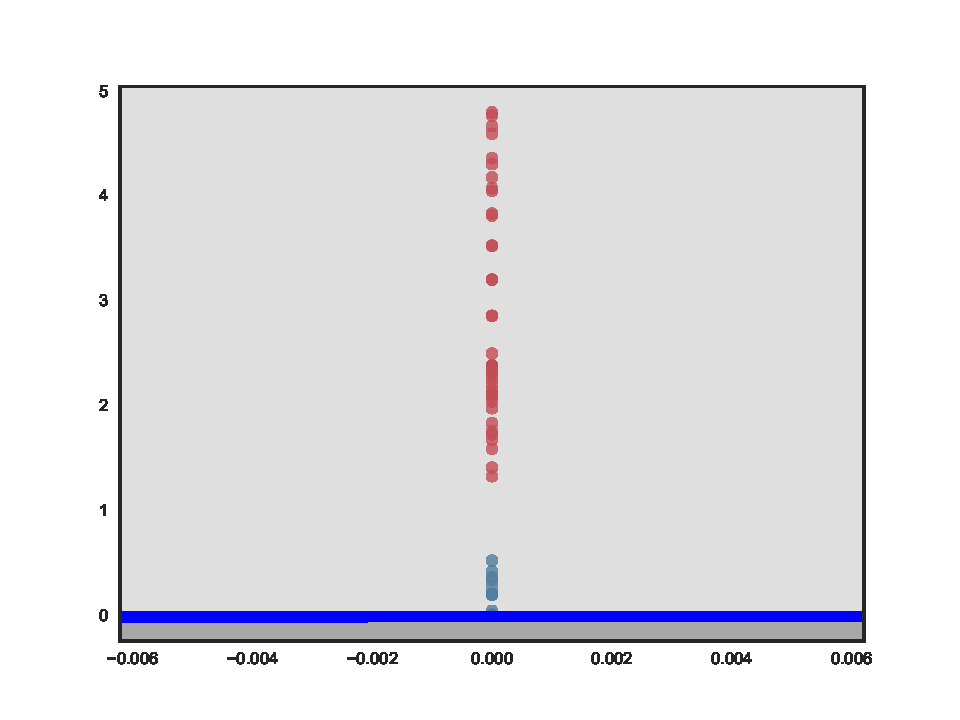
\includegraphics[width=\hsize]{img/toy/unitpointwise/conv2d_4-0.pdf}}
    %   \vskip1em
      \subcaptionbox{4th layer\label{fig:moonsUnitpointwise42}}{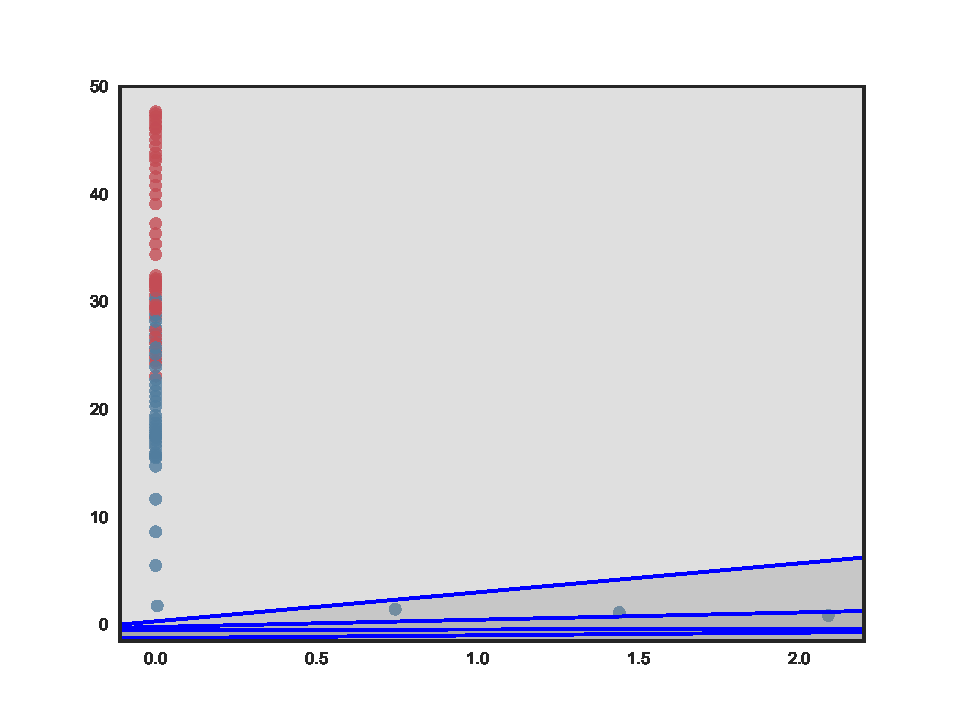
\includegraphics[width=\hsize]{img/toy/unitpointwise/conv2d_4-2.pdf}} 
    }
    % \hskip1em
    \parbox{.195\textwidth}{%
      \subcaptionbox{25th layer\label{fig:moonsUnitpointwise251}}{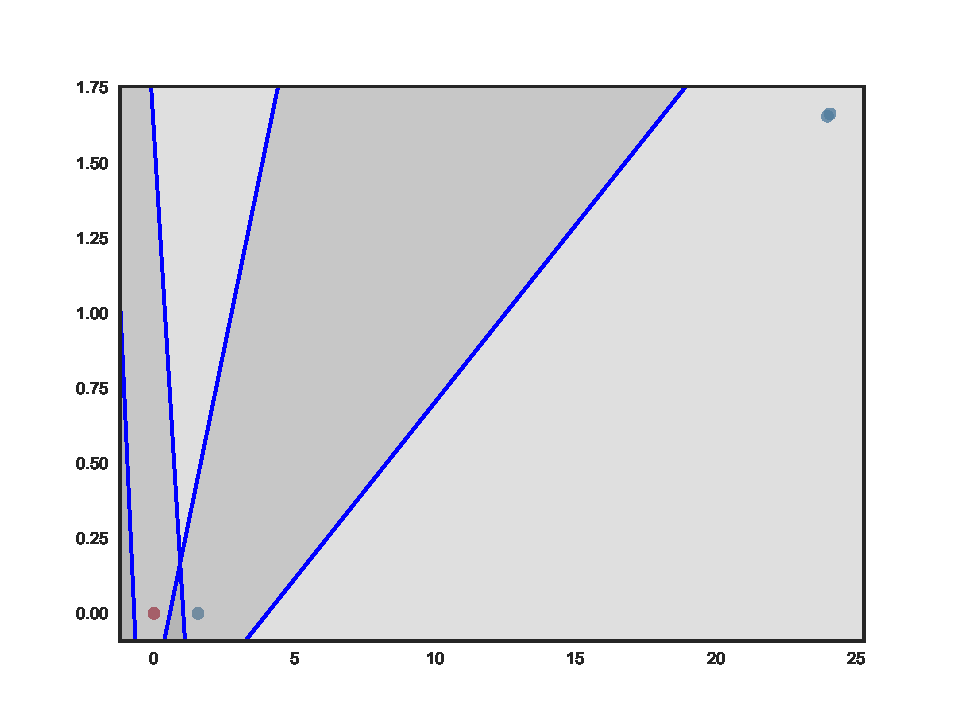
\includegraphics[width=\hsize]{img/toy/unitpointwise/conv2d_25-0.pdf}}
    %   \vskip1em
      \subcaptionbox{25th layer\label{fig:moonsUnitpointwise252}}{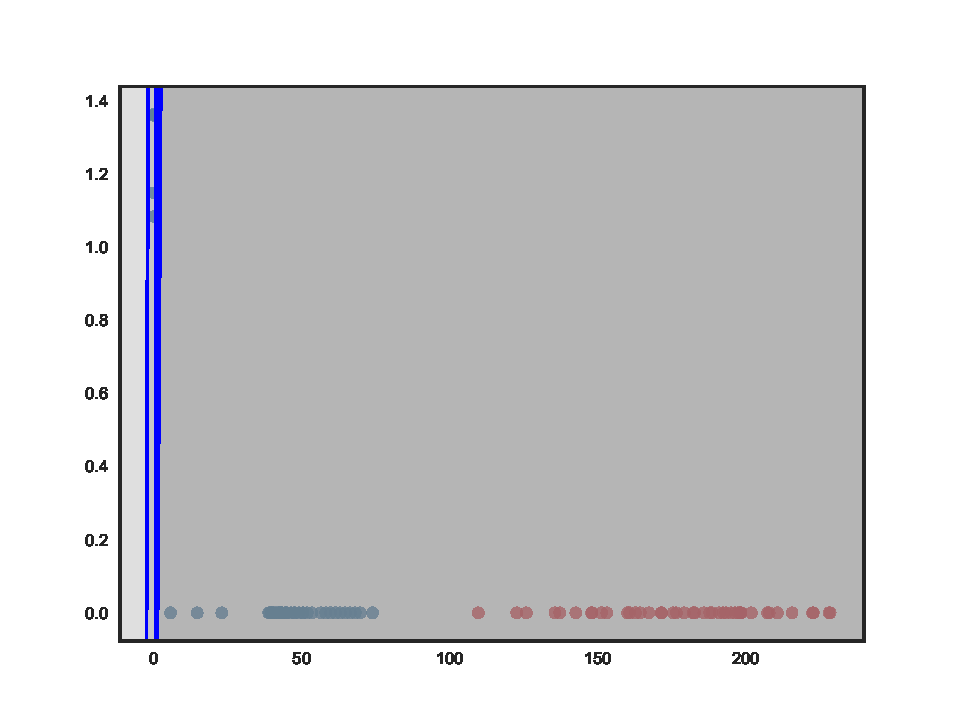
\includegraphics[width=\hsize]{img/toy/unitpointwise/conv2d_25-2.pdf}} 
    }
    % \hskip1em
    \parbox{.195\textwidth}{%
      \subcaptionbox{Feature layer\label{fig:moonsUnitpointwiseFeature1}}{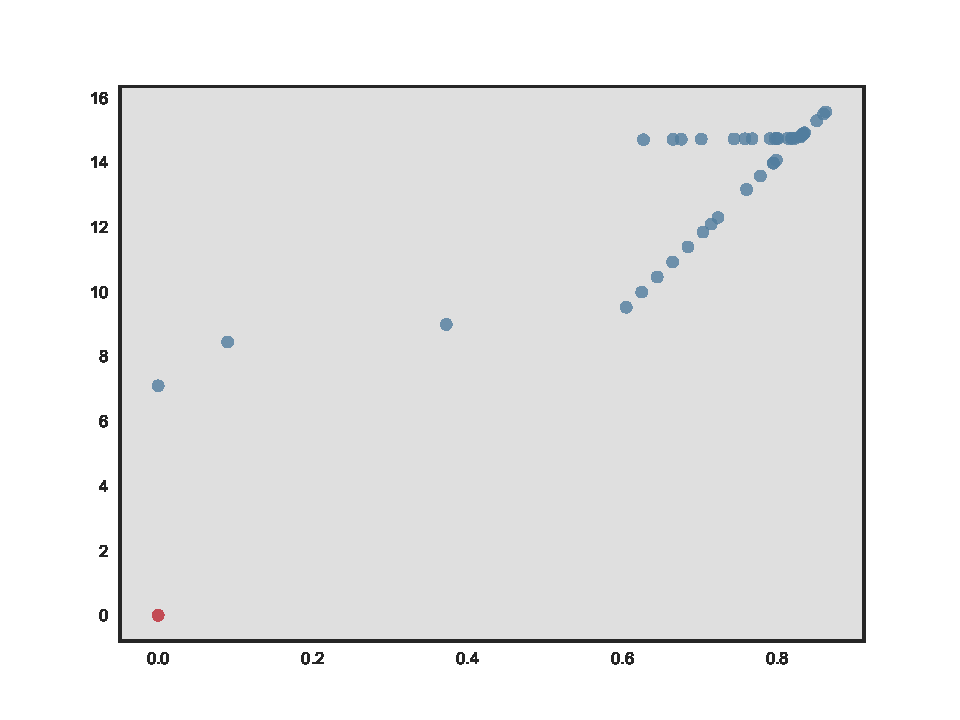
\includegraphics[width=\hsize]{img/toy/unitpointwise/dense_1-0.pdf}}
    %   \vskip1em
      \subcaptionbox{Feature layer\label{fig:moonsUnitpointwiseFeature2}}{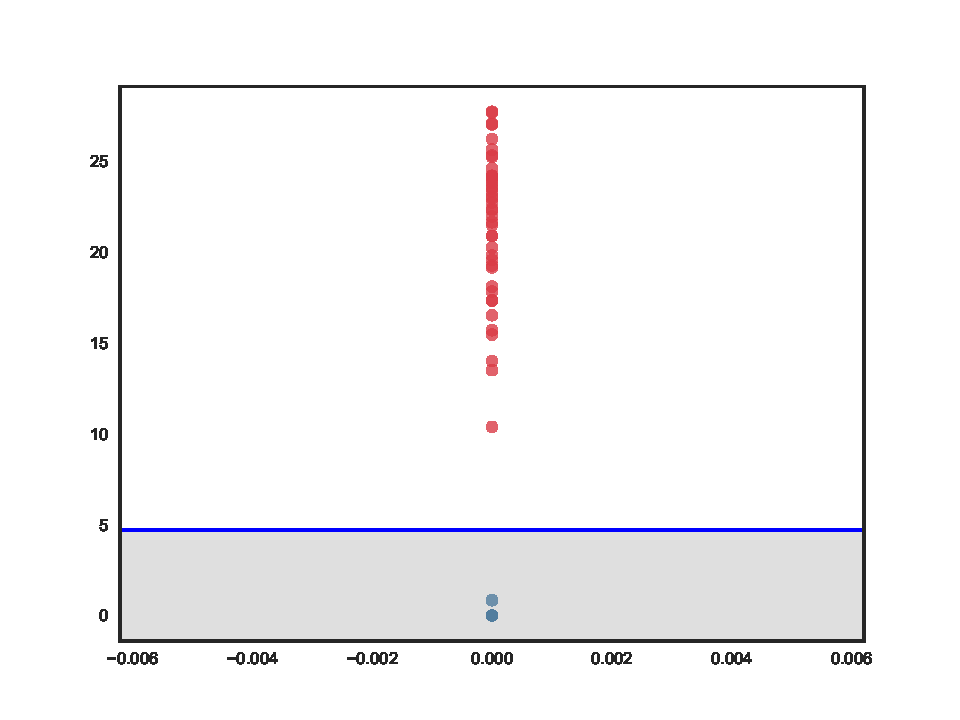
\includegraphics[width=\hsize]{img/toy/unitpointwise/dense_1-2.pdf}} 
    }
    % \hskip1em
    \parbox{.195\textwidth}{%
      \subcaptionbox{Output\label{fig:moonsUnitpointwiseOutput}}{
      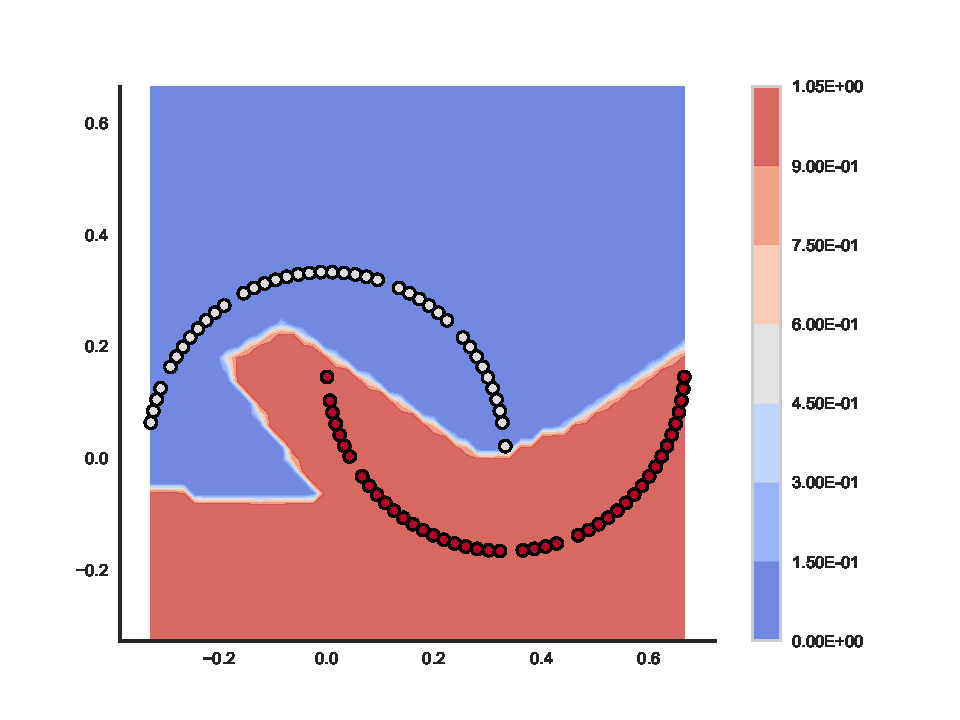
\includegraphics[clip, trim=2.35cm 1.75cm 4.5cm 0cm,width=\hsize, height=\hsize]{img/toy/unitpointwise/output.pdf}
      }
    }
  }

    \caption{Data transformed across a 50x4 \SepUnitPoint network. The network displays internal representations without collapsing the dataset like \SepPoint while retaining classification power like \SepUnit.}
    \label{fig:moonsUnitPointwise}
\end{figure*}

\begin{figure*}[h!]
  \centering
  \parbox{\textwidth}{
    \parbox{.195\textwidth}{%
      \subcaptionbox{Input layer\label{fig:moonsLayerwiseInput}}{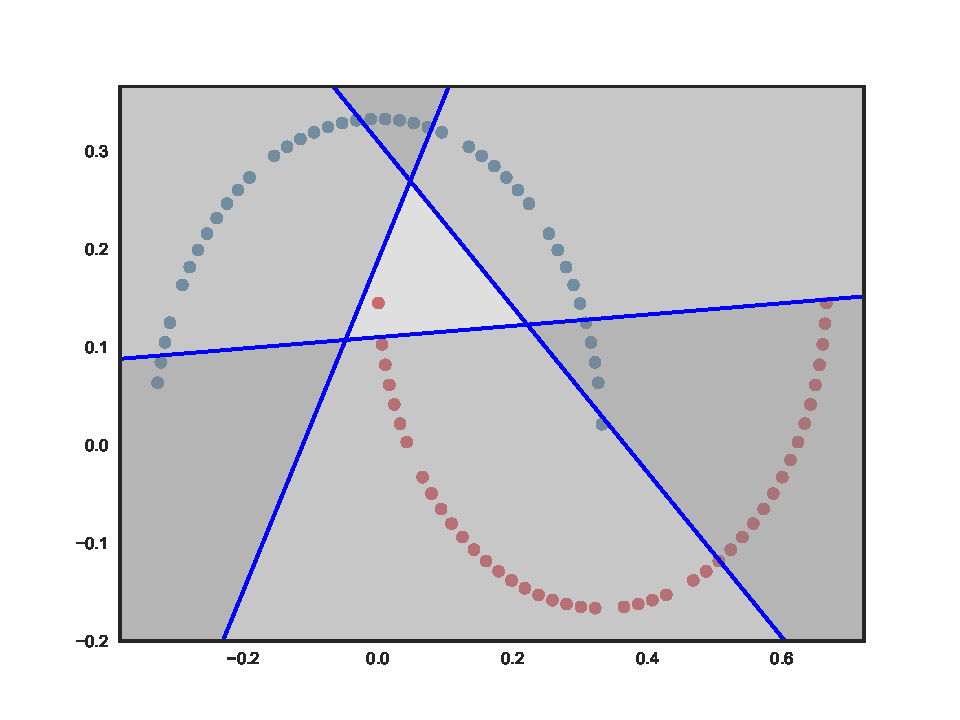
\includegraphics[width=\hsize]{img/toy/layerwise/conv2d_1-0.pdf}}
    }
    % \hskip1em
    \parbox{.195\textwidth}{%
      \subcaptionbox{4th layer\label{fig:moonsLayerwise41}}{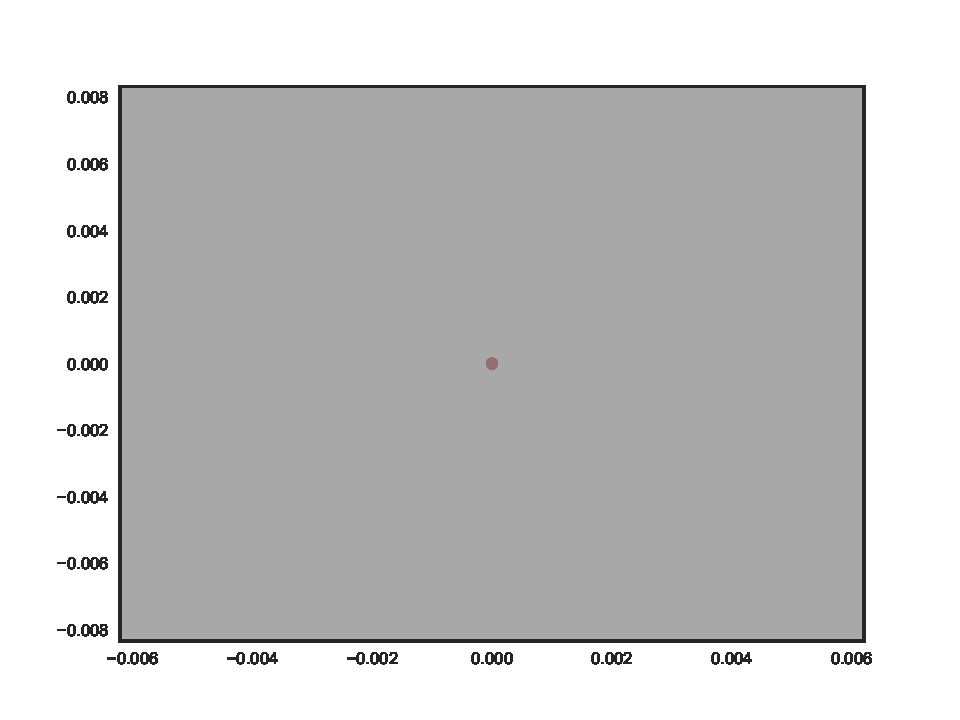
\includegraphics[width=\hsize]{img/toy/layerwise/conv2d_4-0.pdf}}
    %   \vskip1em
      \subcaptionbox{4th layer\label{fig:moonsLayerwise42}}{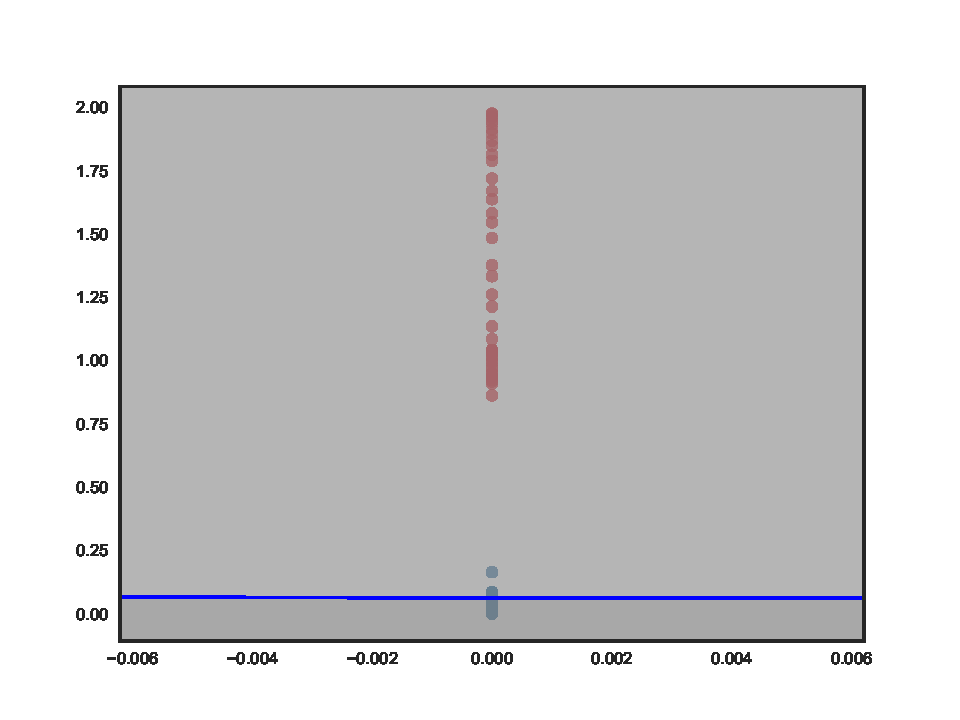
\includegraphics[width=\hsize]{img/toy/layerwise/conv2d_4-2.pdf}} 
    }
    % \hskip1em
    \parbox{.195\textwidth}{%
      \subcaptionbox{25th layer\label{fig:moonsLayerwise251}}{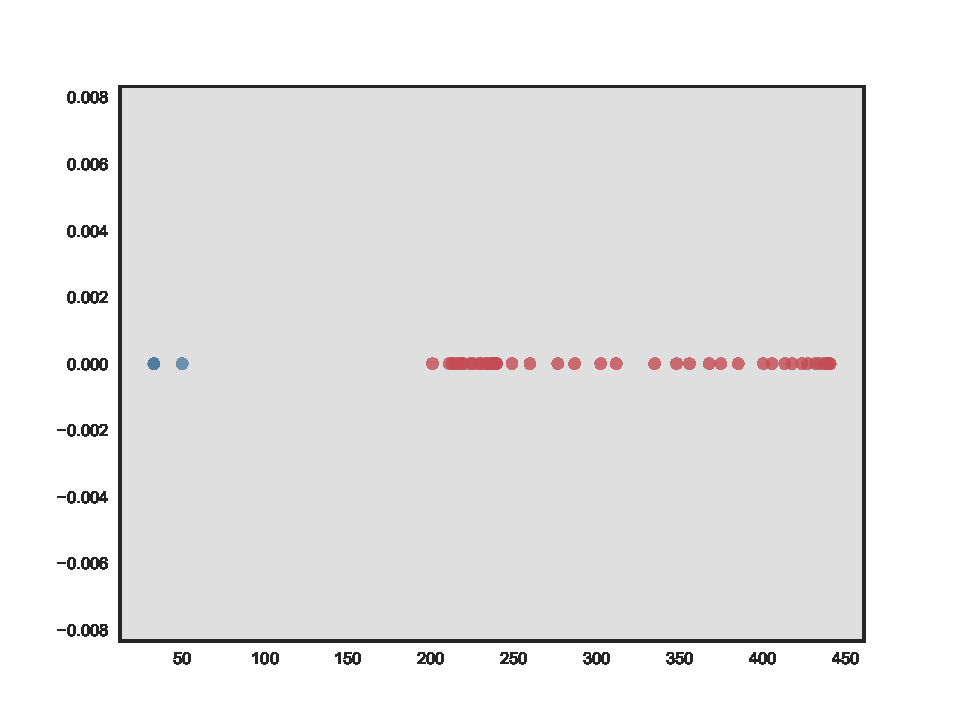
\includegraphics[width=\hsize]{img/toy/layerwise/conv2d_25-0.pdf}}
    %   \vskip1em
      \subcaptionbox{25th layer\label{fig:moonsLayerwise252}}{\includegraphics[width=\hsize]{img/toy/layerwise/conv2d_25-2.pdf}} 
    }
    % \hskip1em
    \parbox{.195\textwidth}{%
      \subcaptionbox{Feature layer\label{fig:moonsLayerwiseFeature1}}{\includegraphics[width=\hsize]{img/toy/layerwise/dense_1-0.pdf}}
    %   \vskip1em
      \subcaptionbox{Feature layer\label{fig:moonsLayerwiseFeature2}}{\includegraphics[width=\hsize]{img/toy/layerwise/dense_1-2.pdf}} 
    }
    % \hskip1em
    \parbox{.195\textwidth}{%
      \subcaptionbox{Output\label{fig:moonsLayerwiseOutput}}{\includegraphics[clip, trim=2.35cm 1.75cm 4.5cm 0cm,width=\hsize]{img/toy/layerwise/output.pdf}}
    }
  }
    \caption{Data transformed across a 50x4 \SepLayer network. Although being a relaxation of \SepUnitPoint showing an intuitive solution with several affine and dead units. Indeed, they not only do not hinder the network but forward the solution 4th layer to the output.}
    \label{fig:moonsLayerwise}
\end{figure*}

\begin{figure*}[h!]
  \centering
    \begin{subfigure}[b]{0.3\textwidth}
        \includegraphics[width=\textwidth]{img/init/relu/conv2d_1-0.pdf}
        \caption{\ReLU input layer}
        \label{fig:reluInitInput}
    \end{subfigure}
    ~ %add desired spacing between images, e. g. ~, \quad, \qquad, \hfill etc. 
      %(or a blank line to force the subfigure onto a new line)
    \begin{subfigure}[b]{0.3\textwidth}
        \includegraphics[width=\textwidth]{img/init/relu/conv2d_50-0.pdf}
        \caption{\ReLU 50th layer}
        \label{fig:reluInit501}
    \end{subfigure}
    ~ %add desired spacing between images, e. g. ~, \quad, \qquad, \hfill etc. 
    %(or a blank line to force the subfigure onto a new line)
    \begin{subfigure}[b]{0.3\textwidth}
        \includegraphics[width=\textwidth]{img/init/relu/conv2d_50-2.pdf}
        \caption{\ReLU 50th layer}
        \label{fig:reluInit502}
    \end{subfigure}
    \\
    \begin{subfigure}[b]{0.3\textwidth}
        \includegraphics[width=\textwidth]{img/init/relu-bn/conv2d_1-0.pdf}
        \caption{\ReLUBN input layer}
        \label{fig:reluBNInitInput}
    \end{subfigure}
    ~ %add desired spacing between images, e. g. ~, \quad, \qquad, \hfill etc. 
      %(or a blank line to force the subfigure onto a new line)
    \begin{subfigure}[b]{0.3\textwidth}
        \includegraphics[width=\textwidth]{img/init/relu-bn/conv2d_50-0.pdf}
        \caption{\ReLUBN 50th layer}
        \label{fig:reluBNInit501}
    \end{subfigure}
    ~ %add desired spacing between images, e. g. ~, \quad, \qquad, \hfill etc. 
    %(or a blank line to force the subfigure onto a new line)
    \begin{subfigure}[b]{0.3\textwidth}
        \includegraphics[width=\textwidth]{img/init/relu-bn/conv2d_50-2.pdf}
        \caption{\ReLUBN 50th layer}
        \label{fig:reluBNInit502}
    \end{subfigure}
    \\
    \begin{subfigure}[b]{0.3\textwidth}
        \includegraphics[width=\textwidth]{img/init/layerwise/conv2d_1-0.pdf}
        \caption{\SepLayer input layer}
        \label{fig:layerwiseInitInput}
    \end{subfigure}
    ~ %add desired spacing between images, e. g. ~, \quad, \qquad, \hfill etc. 
      %(or a blank line to force the subfigure onto a new line)
    \begin{subfigure}[b]{0.3\textwidth}
        \includegraphics[width=\textwidth]{img/init/layerwise/conv2d_50-0.pdf}
        \caption{\SepLayer 50th layer}
        \label{fig:layerwiseInit501}
    \end{subfigure}
    ~ %add desired spacing between images, e. g. ~, \quad, \qquad, \hfill etc. 
    %(or a blank line to force the subfigure onto a new line)
    \begin{subfigure}[b]{0.3\textwidth}
        \includegraphics[width=\textwidth]{img/init/layerwise/conv2d_50-2.pdf}
        \caption{\SepLayer 50th layer}
        \label{fig:layerwiseInit502}
    \end{subfigure}
    \\
    \begin{subfigure}[b]{0.3\textwidth}
        \includegraphics[width=\textwidth]{img/init/unitpointwise/conv2d_1-0.pdf}
        \caption{\SepUnitPoint Input}
        \label{fig:unitpointInitInput}
    \end{subfigure}
    ~ %add desired spacing between images, e. g. ~, \quad, \qquad, \hfill etc. 
      %(or a blank line to force the subfigure onto a new line)
    \begin{subfigure}[b]{0.3\textwidth}
        \includegraphics[width=\textwidth]{img/init/unitpointwise/conv2d_50-0.pdf}
        \caption{\SepUnitPoint 50th layer}
        \label{fig:unitpointInit501}
    \end{subfigure}
    ~ %add desired spacing between images, e. g. ~, \quad, \qquad, \hfill etc. 
    %(or a blank line to force the subfigure onto a new line)
    \begin{subfigure}[b]{0.3\textwidth}
        \includegraphics[width=\textwidth]{img/init/unitpointwise/conv2d_50-2.pdf}
        \caption{\SepUnitPoint 50th layer}
        \label{fig:unitpointInit502}
    \end{subfigure}
    
  \caption{Data transformed across a 50x4 network with no main loss (cross-entropy) with constraints \SepLayer and \SepUnitPoint, versus \ReLU and \ReLUBN. Notice how effectively \ReLU and \ReLUBN collapse the dataset into few points whereas \SepLayer and \SepUnitPoint force the network to learn representations that preserve geometrical structure useful for back-propagation.} 
  \label{fig:init} 
\end{figure*}

\subsection{Dynamic Behavior of the constraints}\label{subsec:dynamicBehavior}
\begin{figure*}[h!]
    \begin{subfigure}[c]{1\textwidth}
        \centering
        \includegraphics[width=1\textwidth]{img/convergence/peaks_loss.pdf}
        \caption{Evolution of cross-entropy and constraint loss during training.}
        \label{fig:loss_convergence}
    \end{subfigure}
    \\
    \begin{subfigure}[c]{1\textwidth}
        \centering
        \begin{tikzpicture}[remember picture]
            \node[anchor=south west,inner sep=0] (loss) at (0,0) {
            \includegraphics[width=1\textwidth]{img/convergence/peaks_acc.pdf}};
        \end{tikzpicture}
        \caption{Evolution of accuracy during training.}
        \label{fig:accuracy_convergence}
    \end{subfigure}
    \\
     
\begin{subfigure}[b]{0.0325\textwidth}
    \begin{tikzpicture}
    \node[remember picture,anchor=south west,inner sep=0] (1154) at (0,0) {\includegraphics[clip, trim=2.35cm 1.75cm 4.5cm 0cm,width=1.1\textwidth]{img/convergence/1154.pdf}};
    \end{tikzpicture}
    \label{fig:convergence_1154}
\end{subfigure}
%
\begin{subfigure}[b]{0.0325\textwidth}
    \includegraphics[clip, trim=2.35cm 1.75cm 4.5cm 0cm,width=1.1\textwidth]{img/convergence/2400.pdf}
    \label{fig:convergence_2400}
\end{subfigure}
%
\begin{subfigure}[b]{0.0325\textwidth}
    \includegraphics[clip, trim=2.35cm 1.75cm 4.5cm 0cm,width=1.1\textwidth]{img/convergence/6200.pdf}
    \label{fig:convergence_6200}
\end{subfigure}
%
\begin{subfigure}[b]{0.0325\textwidth}
    \includegraphics[clip, trim=2.35cm 1.75cm 4.5cm 0cm,width=1.1\textwidth]{img/convergence/6205.pdf}
    \label{fig:convergence_6205}
\end{subfigure}
%
\begin{subfigure}[b]{0.0325\textwidth}
    \includegraphics[clip, trim=2.35cm 1.75cm 4.5cm 0cm,width=1.1\textwidth]{img/convergence/7200.pdf}
    \label{fig:convergence_7200}
\end{subfigure}
%
\begin{subfigure}[b]{0.0325\textwidth}
    \includegraphics[clip, trim=2.35cm 1.75cm 4.5cm 0cm,width=1.1\textwidth]{img/convergence/8123.pdf}
    \label{fig:convergence_8123}
\end{subfigure}
%
\begin{subfigure}[b]{0.0325\textwidth}
    \includegraphics[clip, trim=2.35cm 1.75cm 4.5cm 0cm,width=1.1\textwidth]{img/convergence/8132.pdf}
    \label{fig:convergence_8132}
\end{subfigure}
%
\begin{subfigure}[b]{0.0325\textwidth}
    \includegraphics[clip, trim=2.35cm 1.75cm 4.5cm 0cm,width=1.1\textwidth]{img/convergence/8264.pdf}
    \label{fig:convergence_8264}
\end{subfigure}
%
\begin{subfigure}[b]{0.0325\textwidth}
    \includegraphics[clip, trim=2.35cm 1.75cm 4.5cm 0cm,width=1.1\textwidth]{img/convergence/8344.pdf}
    \label{fig:convergence_8344}
\end{subfigure}
%
\begin{subfigure}[b]{0.0325\textwidth}
    \includegraphics[clip, trim=2.35cm 1.75cm 4.5cm 0cm,width=1.1\textwidth]{img/convergence/9161.pdf}
    \label{fig:convergence_9161}
\end{subfigure}
%
\begin{subfigure}[b]{0.0325\textwidth}
    \includegraphics[clip, trim=2.35cm 1.75cm 4.5cm 0cm,width=1.1\textwidth]{img/convergence/9179.pdf}
    \label{fig:convergence_9179}
\end{subfigure}
%
\begin{subfigure}[b]{0.0325\textwidth}
    \includegraphics[clip, trim=2.35cm 1.75cm 4.5cm 0cm,width=1.1\textwidth]{img/convergence/11883.pdf}
    \label{fig:convergence_11883}
\end{subfigure}
%
\begin{subfigure}[b]{0.0325\textwidth}
    \includegraphics[clip, trim=2.35cm 1.75cm 4.5cm 0cm,width=1.1\textwidth]{img/convergence/11886.pdf}
    \label{fig:convergence_11886}
\end{subfigure}
%
\begin{subfigure}[b]{0.0325\textwidth}
    \includegraphics[clip, trim=2.35cm 1.75cm 4.5cm 0cm,width=1.1\textwidth]{img/convergence/12584.pdf}
    \label{fig:convergence_12584}
\end{subfigure}
%
\begin{subfigure}[b]{0.0325\textwidth}
    \includegraphics[clip, trim=2.35cm 1.75cm 4.5cm 0cm,width=1.1\textwidth]{img/convergence/14000.pdf}
    \label{fig:convergence_14000}
\end{subfigure}
%
\begin{subfigure}[b]{0.0325\textwidth}
    \includegraphics[clip, trim=2.35cm 1.75cm 4.5cm 0cm,width=1.1\textwidth]{img/convergence/14022.pdf}
    \label{fig:convergence_14022}
\end{subfigure}
%
\begin{subfigure}[b]{0.0325\textwidth}
    \includegraphics[clip, trim=2.35cm 1.75cm 4.5cm 0cm,width=1.1\textwidth]{img/convergence/14382.pdf}
    \label{fig:convergence_14382}
\end{subfigure}
%
\begin{subfigure}[b]{0.0325\textwidth}
    \includegraphics[clip, trim=2.35cm 1.75cm 4.5cm 0cm,width=1.1\textwidth]{img/convergence/14457.pdf}
    \label{fig:convergence_14457}
\end{subfigure}
%
\begin{subfigure}[b]{0.0325\textwidth}
    \includegraphics[clip, trim=2.35cm 1.75cm 4.5cm 0cm,width=1.1\textwidth]{img/convergence/14461.pdf}
    \label{fig:convergence_14461}
\end{subfigure}
%
\begin{subfigure}[b]{0.0325\textwidth}
    \includegraphics[clip, trim=2.35cm 1.75cm 4.5cm 0cm,width=1.1\textwidth]{img/convergence/15600.pdf}
    \label{fig:convergence_15600}
\end{subfigure}
%
\begin{subfigure}[b]{0.0325\textwidth}
    \includegraphics[clip, trim=2.35cm 1.75cm 4.5cm 0cm,width=1.1\textwidth]{img/convergence/16424.pdf}
    \label{fig:convergence_16424}
\end{subfigure}
%
\begin{subfigure}[b]{0.0325\textwidth}
    \includegraphics[clip, trim=2.35cm 1.75cm 4.5cm 0cm,width=1.1\textwidth]{img/convergence/16432.pdf}
    \label{fig:convergence_16432}
\end{subfigure}
%
\begin{subfigure}[b]{0.0325\textwidth}
    \includegraphics[clip, trim=2.35cm 1.75cm 4.5cm 0cm,width=1.1\textwidth]{img/convergence/16435.pdf}
    \label{fig:convergence_16435}
\end{subfigure}
%
\begin{subfigure}[b]{0.0325\textwidth}
    \includegraphics[clip, trim=2.35cm 1.75cm 4.5cm 0cm,width=1.1\textwidth]{img/convergence/16442.pdf}
    \label{fig:convergence_16442}
\end{subfigure}
%
\begin{subfigure}[b]{0.0325\textwidth}
    \includegraphics[clip, trim=2.35cm 1.75cm 4.5cm 0cm,width=1.1\textwidth]{img/convergence/16444.pdf}
    \label{fig:convergence_16444}
\end{subfigure}
%
\begin{subfigure}[b]{0.0325\textwidth}
    \includegraphics[clip, trim=2.35cm 1.75cm 4.5cm 0cm,width=1.1\textwidth]{img/convergence/16630.pdf}
    \label{fig:convergence_16630}
\end{subfigure}
%
\begin{subfigure}[b]{0.0325\textwidth}
    \includegraphics[clip, trim=2.35cm 1.75cm 4.5cm 0cm,width=1.1\textwidth]{img/convergence/16632.pdf}
    \label{fig:convergence_16632}
\end{subfigure}
%
      \caption{Evolution of training throughout epochs (cross-entropy, constraint loss, and accuracy). Left-hand axis show the accuracy metric (blue line) against the cross-entropy, and constraint loss in the right axis (orange line), for each epoch of the training phase in the horizontal axis.}
	\label{fig:peaks}
\end{figure*}
\begin{figure*}[h!]
  \centering
  \begin{subfigure}[b]{0.2\textwidth}
        \includegraphics[width=\textwidth]{img/moons_grid/acc-sep-up-0-0001.pdf}
        \caption{Glorot initialization}
        \label{fig:moons_glorot_rho}
    \end{subfigure}
    ~ %add desired spacing between images, e. g. ~, \quad, \qquad, \hfill etc. 
      %(or a blank line to force the subfigure onto a new line)
      \centering
    \begin{subfigure}[b]{0.2\textwidth}
        \includegraphics[width=\textwidth]{img/moons_grid/acc-sep-up-0-0001-zero.pdf}
        \caption{Zero initialization with $\rho = 0.51$}
        \label{fig:moons_zeros_rho}
    \end{subfigure}
    ~ %add desired spacing between images, e. g. ~, \quad, \qquad, \hfill etc. 
      %(or a blank line to force the subfigure onto a new line)
    \centering
    \begin{subfigure}[b]{0.2\textwidth}
        \includegraphics[width=\textwidth]{img/moons_grid/acc-sep-up-0-0001-nm-0.pdf}
        \caption{Glorot initialization with negative margin to zero}
        \label{fig:moons_glorot_nm0}
    \end{subfigure}
    ~ %add desired spacing between images, e. g. ~, \quad, \qquad, \hfill etc. 
      %(or a blank line to force the subfigure onto a new line)
    \centering
    \begin{subfigure}[b]{0.2\textwidth}
        \includegraphics[width=\textwidth]{img/moons_grid/acc-sep-up-0-0001-nm-0.pdf}
        \caption{Zero initialization with negative margin to zero}
        \label{fig:moons_zeros_nm0}
    \end{subfigure}
    
  \caption{Glorot vs Zero initialization in a series of Depth $D$ vs Width $W$ accuracy plots a for rectangular network using a grid ($2\leq W\leq 25$ and $2\leq D\leq 150$), trained over the \texttt{MOONS} dataset using an Adam learning rate of $0.01$, annealed dropout for $1000$ epoch with an initial rate of $0.01$ in the. The color scheme depicts accuracy attained for each grid location, from dark to light. (a) classical Glorot, (b) Zero intialization using $\rho=0.51$, (c) Glorot initialization using $\rho=0$ or enforcing only non-negative constraints and (d) Zero initialization using $\rho=0$ or non-negative constraints. 
  }
  \label{fig:moons_grid_zero} 
\end{figure*}
     
\section{Conclusions}\label{sec:conclusions}

% PREGUNTA DEL PAPER
% Since the existing methods require either computational expenditure and add arbitrary complexity to the architecture design, or simply entail limit network performance, we wonder whether we can train deeper networks without relying in any of those techniques. This imply using the minimum width possible, removing any additional connections or activations, and using no normalization. 

% 1.1
The separation constraint is \emph{comparable} to the usual techniques (as presented in the introduction). Indeed, \SepLayer allows for affine units (recall Equation \ref{eq:affineUnit}) that forward representations between layers in the same spirit as ResNets \cite{resnet} or DenseNets \cite{densenet}. Meanwhile, a layer satisfying the \SepPoint constraint ensures the existence of two units with opposite-facing hyperplanes similarly to \texttt{C-ReLU} \cite{crelu}. In addition, the intuition of the separation constraint method intends to serve as stronger heuristic for parameter configuration (independently of initial values), so that units reach a useful configuration for backpropagation, instead of insisting on reaching on some \emph{favorable} initial configuration via trial-and-error as done in the layer-width-increase approach \cite{wideresnet,inceptionv1}.   
\\\\
% 2.1
We claim that there is a difference between non-zero and \emph{useful} activations. As presented in Figure \ref{fig:moonsReLUBN}, \ReLUBN induces a solution that maps the dataset non-trivially throughout the network. However, its performance on the \texttt{MOONS} dataset is inferior to our proposal (63\% of accuracy as presented in Table \ref{tab:moons} against any constraint based test over 90\%). Moreover, comparing the output graph of \ReLUBN (Figure \ref{fig:moonsReLUBNOutput}) with our findings (Figures \ref{fig:moonsUnitwiseOutput}, \ref{fig:moonsPointwiseOutput}. \ref{fig:moonsLayerwiseOutput} and \ref{fig:moonsUnitpointwiseOutput}) the reader can observe that the separation reached separates components of the \texttt{MOONS} dataset in intuitive manners.  
\\\\
% 3.1
The separation constraints compels the data to go through the network favorably for the cross-entropy loss back-propagation. Experimentally, Figure \ref{fig:peaks} suggests that the training phase begins with minimizing the constraint loss until a certain level (approximately $0.21$ around epoch 750), enabling the optimization of the main loss (recall 80 to 100\% accuracy in our tests in Table \ref{tab:moons}). Analytically, we can elaborate on this behavior if we are reminded of the fact that the gradient of the main loss is non-zero \emph{on} the upper sets of units by virtue of Equation \ref{eq:upperPartOfUnit} and the separability conditions presented in subsection \ref{subsec:ReLUSeparability}. Thus, ensuring non-empty upper sets of units is a sufficient condition for back-propagation. 
\\\\
However, further inquiry into the interaction between constraint loss and main loss beyond parameter $\lambda$ is needed. Anecdotal evidence shows spurious transient states on convergence in the cases of \SepPoint, \SepUnit and \SepUnitPoint, but not on \SepLayer.  Additionally, in the scope of our experimentation we have chosen the cross-entropy loss functional, further inquiry is required on the choice of main loss. Another topic that demands further investigation is the use of the separation constraints in other types of layers such as convolutional \cite{lenet}, LSTM \cite{lstm} or transformers \cite{transformer}\cite{transformer2}; other types of tasks such as regression, unsupervised learning, \cite{embedding} graph \cite{graph} or generation \cite{gan}\cite{vae}; and especially more challenging datasets.
\\\\
% 4.1
While the separation constraints prevent the vanishing gradient, the \emph{exploding gradient} remains at large. Notice that the constraints designed place \emph{lower bounds} on the magnitude of the pre-activation values, it places no upper bound. Analytically, this gradient depends on both on the magnitude of the weight vectors, absolute value of the biases and  the magnitude of dataset points mapped throughout the network. This could be solved introducing additional constraints or limiting the norms of weight vectors. 
\\\\
Despite the fact that we intended to avoid dead and affine neurons with our geometrical formulation (recall the predicate $R_1(u) \wedge R_2(u)$ defined on Equation XXX) the different constraints  object in practice. While $R_1(u) \wedge R_2(u)$ is valid within \SepUnit and from it, it extends to layers, \SepLayer and \SepPoint,  allow at least on unit to be affine  over the dataset (recall Equation \ref{eq:affineUnit}) and at least another to be dead (recall Equation \ref{eq:deadNeuronVersion2}), invalidating $R_1(u) \wedge R_2(u)$ for each unit in a layer $\layer$, but holding $R_1(\layer) \wedge R_2(\layer)$. 
\\\\
In this sense, neither \emph{repeated} (producing the same upper set), affine nor dead units are \emph{harmful} for network performance, beyond burdening networks with additional non used parameters. They seem ubiquitous in the extent of our experimentation as Figures \ref{fig:moonsLayerwise}, \ref{fig:moonsPointwise} and \ref{fig:moonsUnitpointwise} testify (see the axis-aligned or diagonally expanding intermediate representations of the dataset). Further inquiry is needed to understand how dead, affine and repeated neurons coalesce in solving the problem. In addition, our experimentation suggests that the  the distribution of dead, affine and repeated units varies according to constraint type (in the extent of our experimentation). 
\\\\
Indeed, Figure \ref{fig:moonsLayerwise} for the \SepLayer constraint type showcases a feature layer (divisions \ref{fig:moonsLayerwiseFeature1} and \ref{fig:moonsLayerwiseFeature1}) with two dead units and two repeated. Meanwhile Figure \ref{fig:moonsUnitwise} at the 24th layer (divisions \ref{fig:moonsUnitwise251} and \ref{fig:moonsUnitwise252}), depicts repeated neurons (organized pairwise) with no affine nor dead units. 
\\\\
Analytically, we can approach affine units in the same spirit as \texttt{ResNet} \cite{resnet} or \texttt{DenseNet}\cite{densenet}. Since the composition of affine functions is affine, collections of successive (across the layers) affine units effectively \emph{shortcut} the network. Experimentally, we verify this in our \SepLayer experiments (as it is the only separation constraint that allows affine units). Notice that there is a coalescence between axis-aligned and diagonal units that preserves the topology of the intermediate representation of the dataset after layer 4, see Figures \ref{fig:moonsLayerwise42} and \ref{fig:moonsLayerwiseFeature2} are almost equal. We conjecture that repeated units perform the same role for \SepUnit, since affine units are forbidden with this constraint. Notice how in Figure \ref{fig:moonsUnitwise252} all the planes are cutting at the same point, thus having the same \emph{upper} and \emph{lower} sets. Interestingly, those sets are compressed into two points in the feature layer (Figures \ref{fig:moonsUnitwiseFeature1} and \ref{fig:moonsUnitwiseFeature2}), but if we add \SepPoint as in \SepUnitPoint we find the same behaviour again, where the feature layer is similar to the inner representation at layer 25 (Figures \ref{fig:moonsUnitpointwise252} and \ref{fig:moonsUnitpointwiseFeature2}). 
\\\\
We explore the use of separation constraint (\SepUnitPoint in this case) to enable zero initialization with good results, see Section \ref{subsec:zero}. In order to make it work though, we had to introduce  means to break the symmetry between the positive and negative constraint ,in the form of $\rho$ (see Equation \ref{eq:definitionOfRho}), and to break symmetry in the weights, in the form of Annealed Dropout \cite{dropoutAnnealing}. Since our objective in this matter (along with all the paper) was simplicity, and the use of Dropout partially defeats this purpose by moving the same stochasticity that we were removing from intialization into training. Nevertheless, our \emph{ansatz} is that an initialization that is based on the data (which is the result of using the constriant plus Dropout) must be superior to any random initialization which is only based in features like gradient magnitude or inputs and outputs. Further research in this matter is hereby required.








{\small
\bibliographystyle{ieee}
\bibliography{egbib}
}

\end{document}
